%!TEX root = ../main.tex

\chapter{Experiments\label{chap:experiments}}

\section{Equipment}

\subsection{UAVs}
The experimental platform for this work was the \ac{MRS} X500~\cite{hertmrs} quadrotor \ac{UAV} equipped with \ac{UV} \ac{LED}s
integrated to the UVDAR system~\cite{walteruvdar}.
Each of the \ac{UAV}'s arms was equipped with 2 \ac{UV} \ac{LED}s at each end of the arm, placed at a right angle relative to each other.
The \ac{LED}s on each arm could be modulated
by using a binary sequence (for example, $"0, 1"$ for simple blinking or $"1"$ for a constant ON signal), with a common modulation frequency set for all the \ac{LED}s.
In our approach, this functionality was used to differentiate between the arms by modulating each arm on a different frequency to be easily distinguishable.
The \ac{UAV} can be seen in \reffig{fig:uav1}.
%\begin{figure}[H]
%    \centering
%    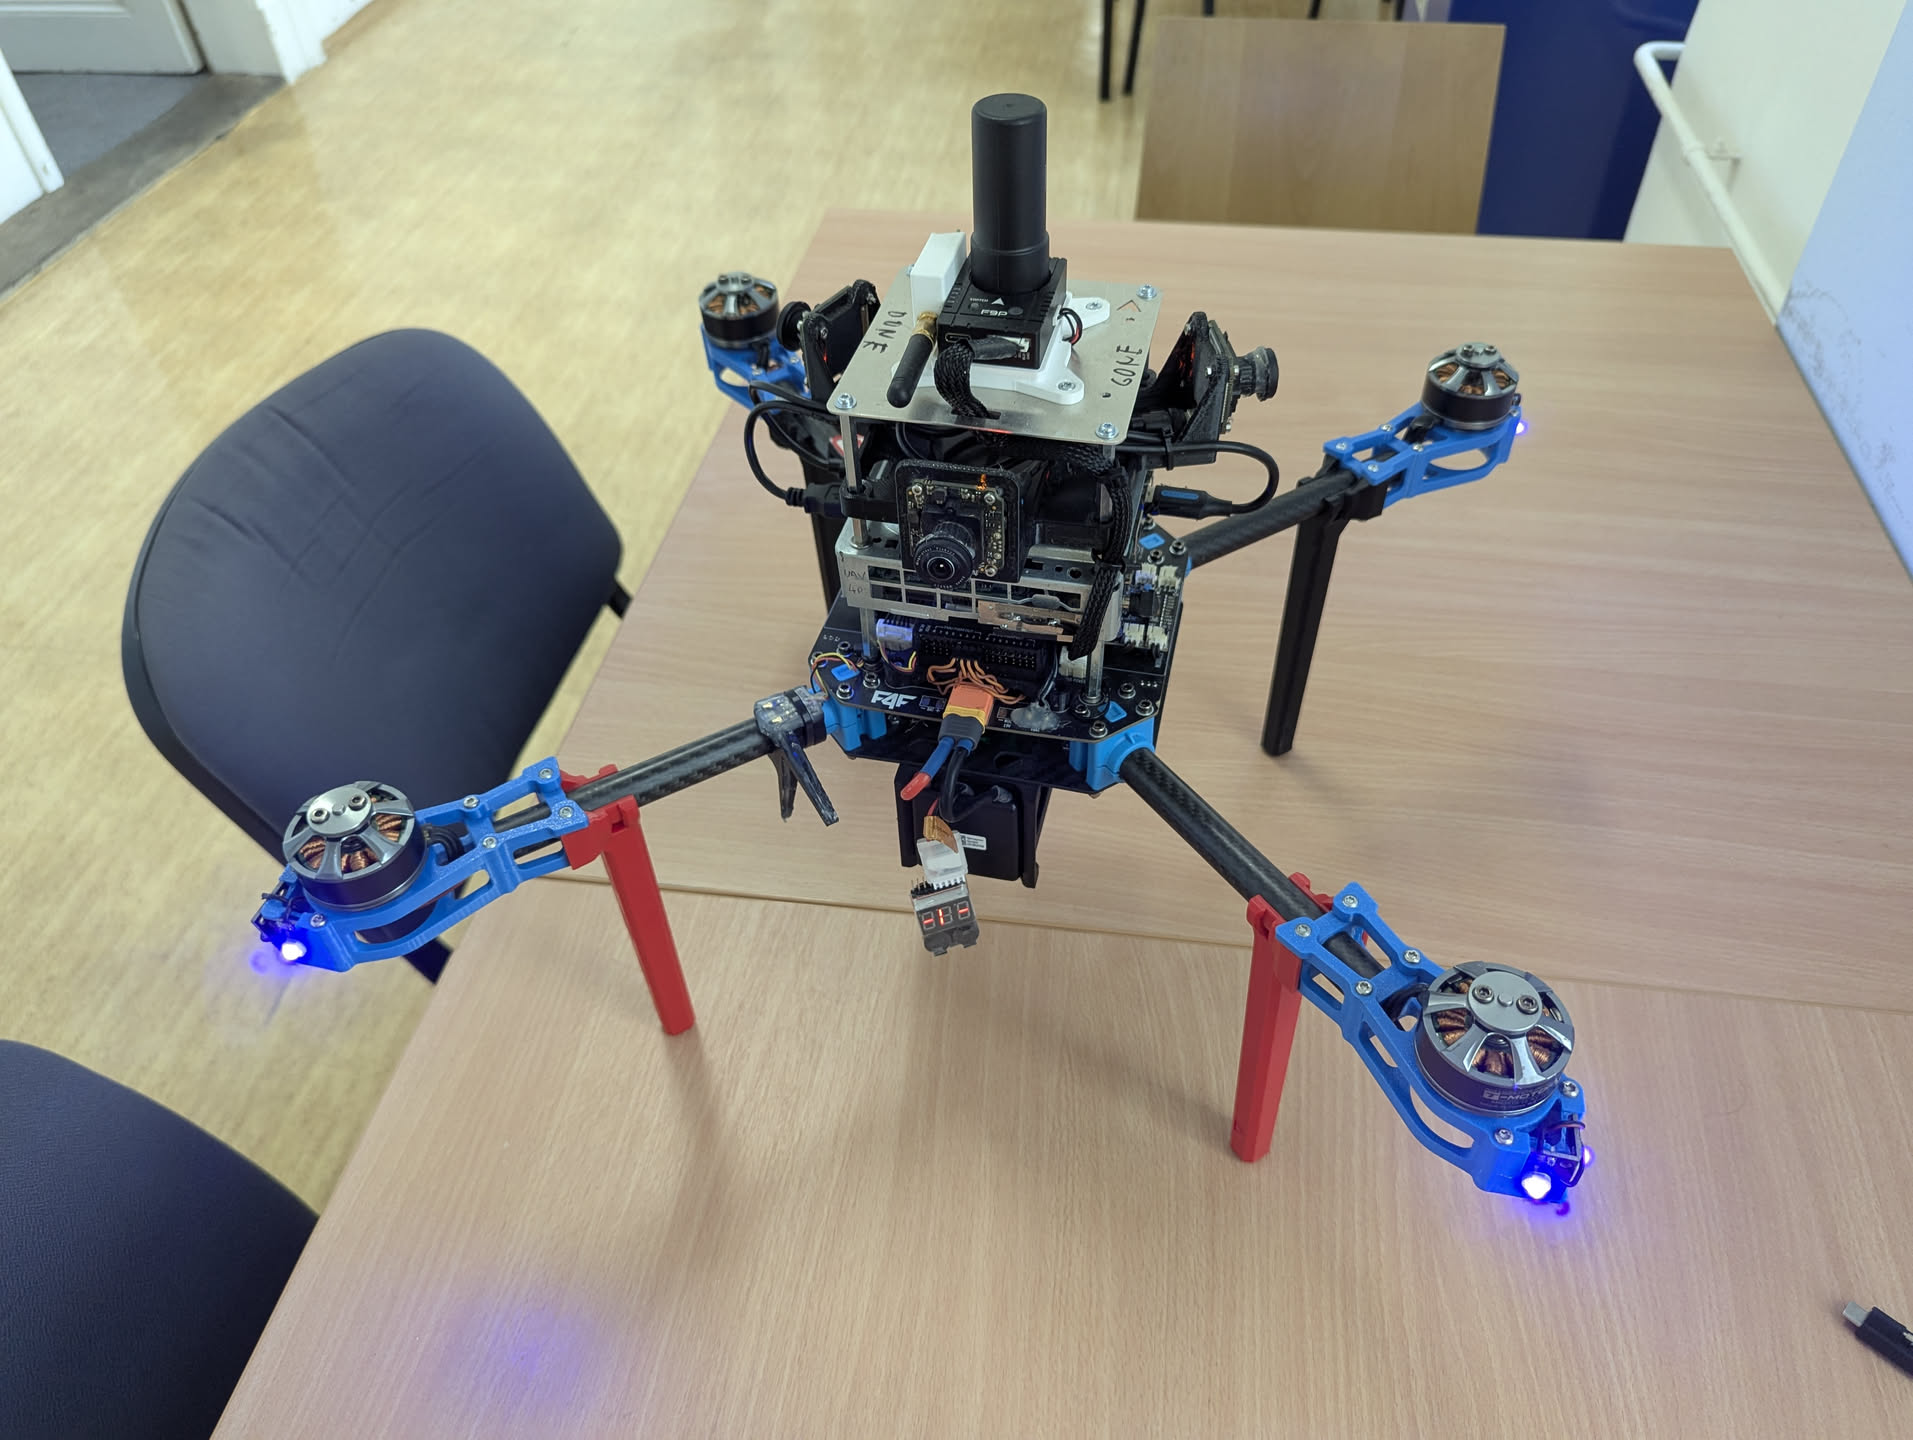
\includegraphics[width=0.50\textwidth]{./fig/photos/uav1.jpeg}
%    \caption{
%        The MRSX500 UAV
%    }
%    \label{fig:x500uav}
%\end{figure}

\subsection{Event-based camera}
The event-based camera used in this thesis was the \texttt{Prophesee EVK4 HD}\footnote{Prophesee EVK4 HD website: \url{https://www.prophesee.ai/event-camera-evk4/}.}~\cite{propheseeevk4},
with \texttt{IMX636} sensor. The camera featured a resolution of $1280 \times 720$ pixels and is capable of generating $1.066\ \text{Gev}/\text{s}$,
although limited by the USB3 interface to $\sim 150\ \text{Mev}/\text{s}$, and offered a dynamic range of $120$ dB.
%\begin{figure}[H]
%    \centering
%    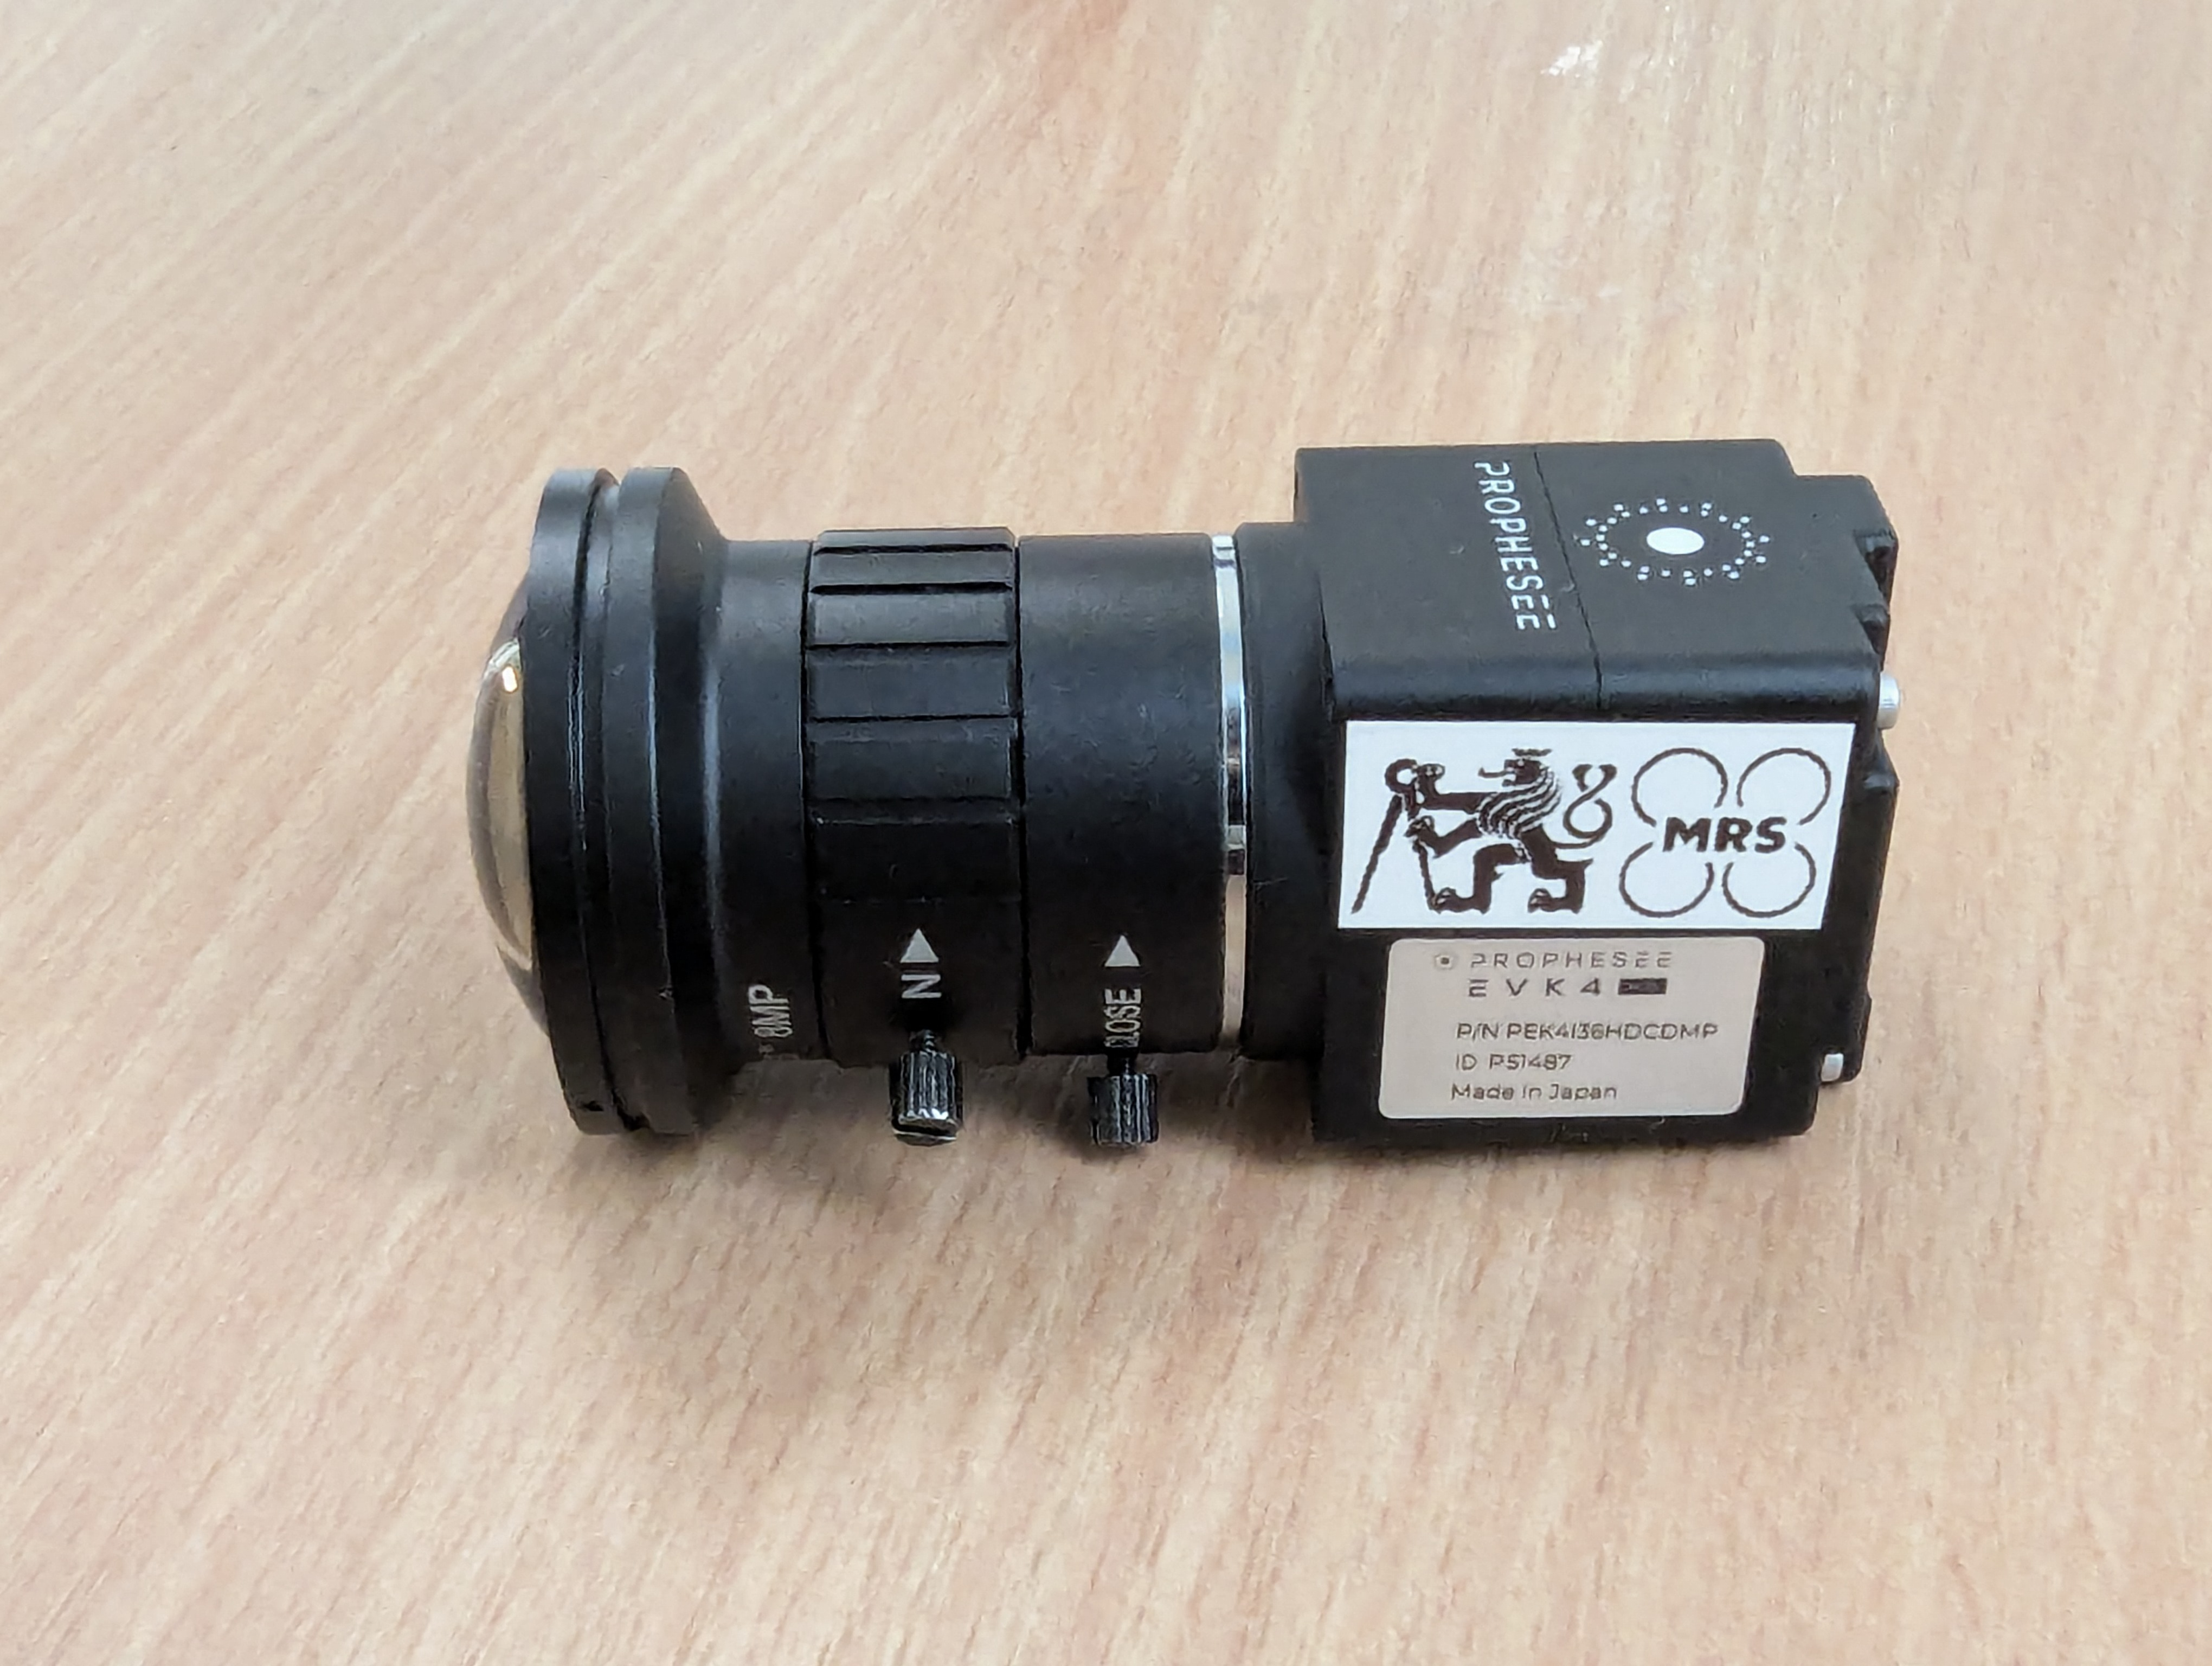
\includegraphics[width=0.50\textwidth]{./fig/photos/evk4.jpg}
%    \caption{
%        Prophesee EVK4 HD event-based camera
%    }
%    \label{fig:evk4}
%\end{figure}

\begin{figure}[H]
	\centering
	\subfloat[The event-based camera EVK4 from Prophesee with a 2.5mm fisheye lens.] {
	  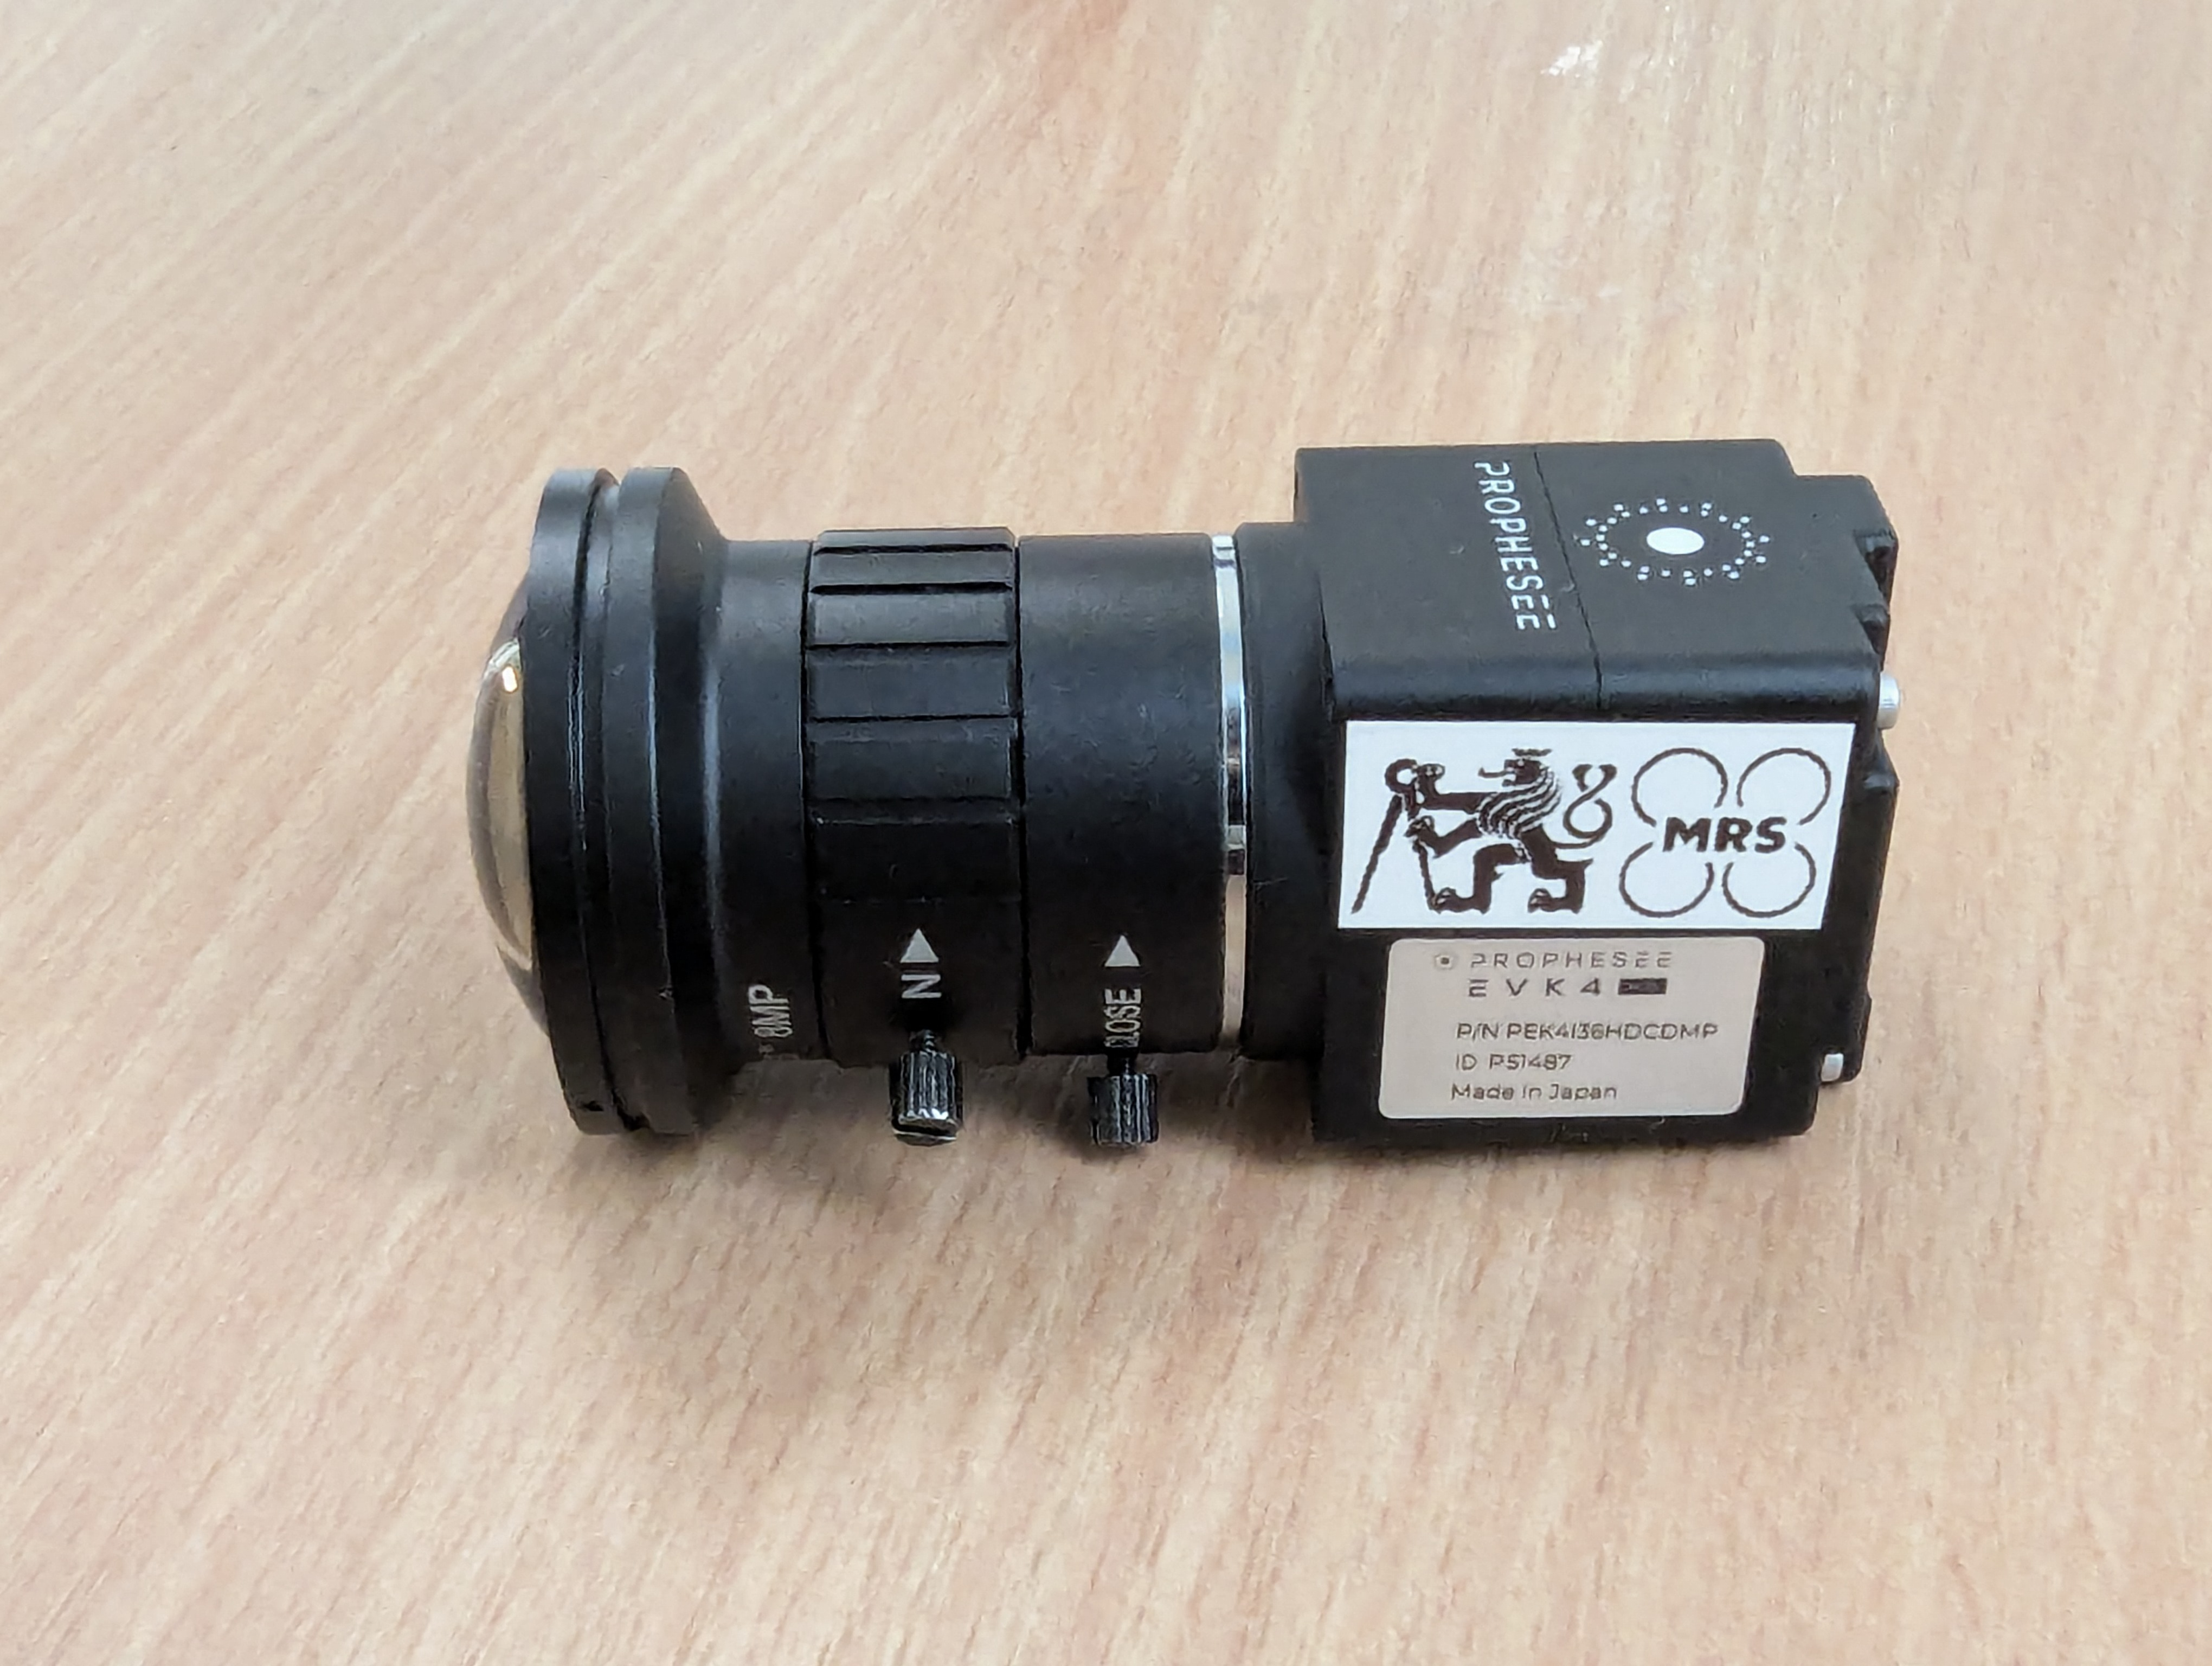
\includegraphics[width=0.5\textwidth]{./fig/photos/evk4.jpg}
	  \label{fig:evk4}
	}
	\subfloat[X500 UAV unit equipped with UVDAR] {
	  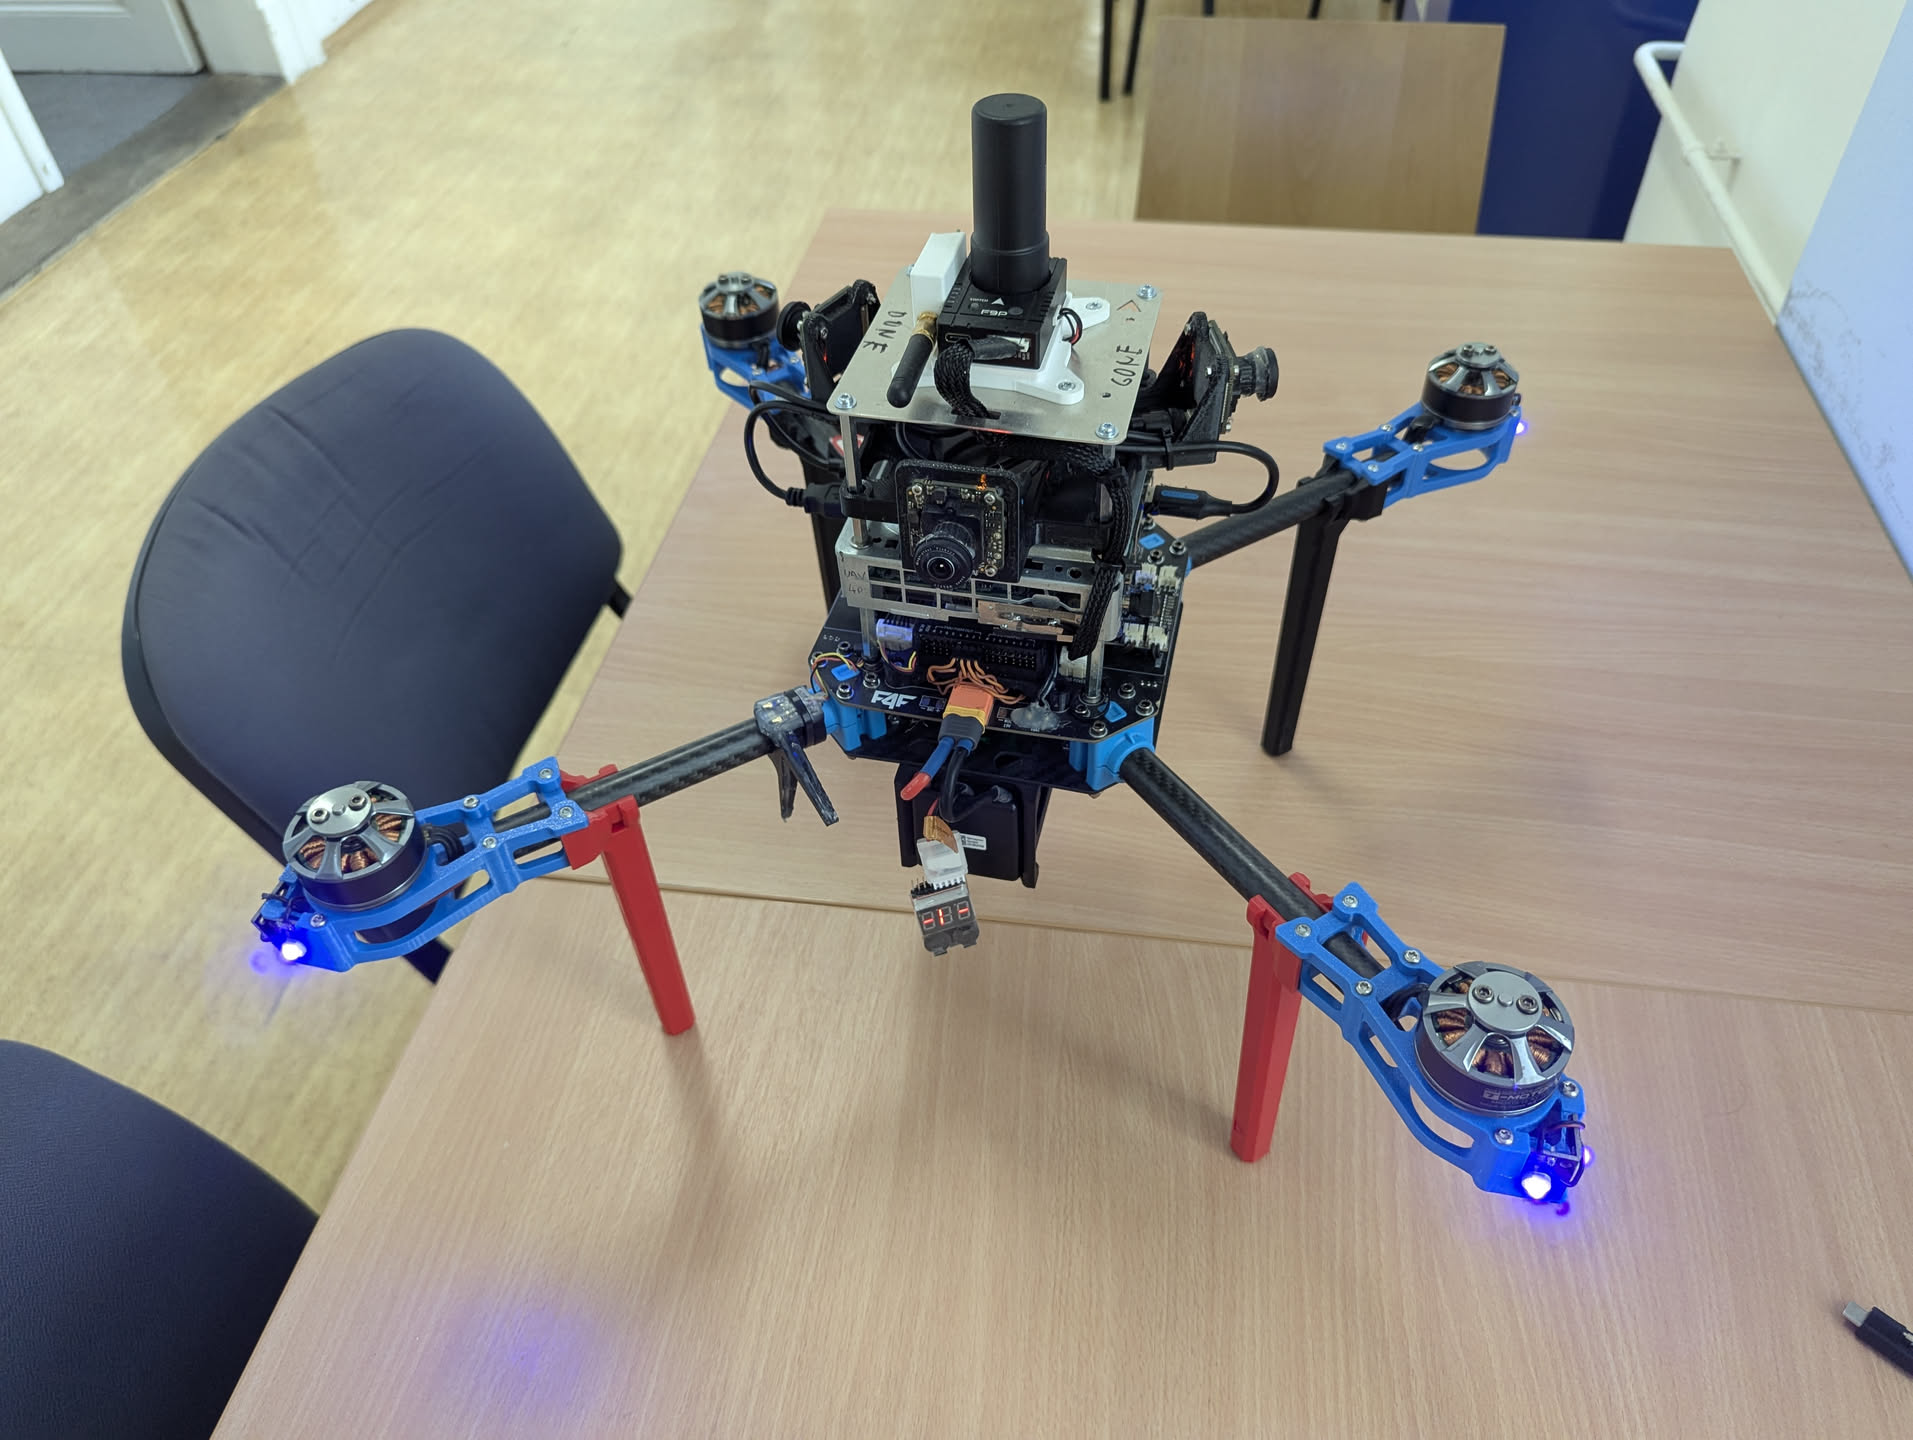
\includegraphics[width=0.5\textwidth]{./fig/photos/uav1.jpeg}
	  \label{fig:uav1}
	}
	\caption{
  An event-based camera with a 2.5mm fisheye lens can be seen on \reffig{fig:evk4}, which was used to measure the UV LEDs mounted on the X500 UAV unit modulated using UVDAR as seen on \reffig{fig:uav1}.
  }
	\label{fig:uavcam}
\end{figure}

\subsection{Lenses}
During the measurements, fisheye lens with a focal length of $2.5$mm and the maximum aperture of f/$1.6$ with \ac{FOV} of $187$ degrees was used. Subsequently, during the real life experiment, an ultra-wide $1.07$mm f/$2.8$ fisheye lens from Entaniya with \ac{FOV} of $280$ degrees was used in combination with the first lens. Both lenses can be seen on \reffig{fig:lenses}.
The lenses were equipped with narrowband \ac{UV} filters which target the specific wavelength of the \ac{LED}s that are used in the UVDAR localization system.
This ensured that the majority of generated events came from the \ac{LED} sources mounted at the \ac{UAV}s, and less events came from the surrounding area.
Both lenses were also properly calibrated, which was required to provide correct results in the final pose estimation.
\begin{figure}[H]
	\centering
	\subfloat[2.5mm f/1.6 fisheye lens] {
	  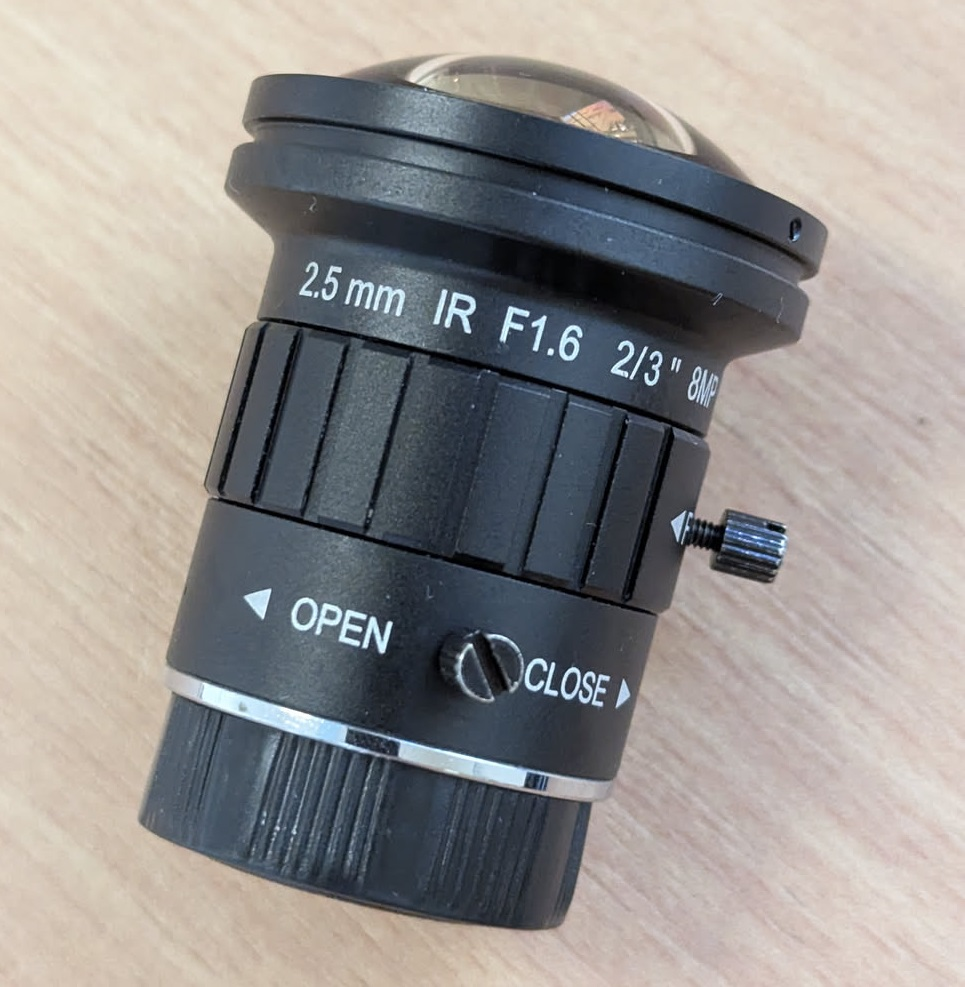
\includegraphics[width=0.391\textwidth]{./fig/photos/lens.jpeg}
	  \label{fig:lens_1}
	}
	\subfloat[1.07mm f/2.8 Entaniya fisheye lens] {
	  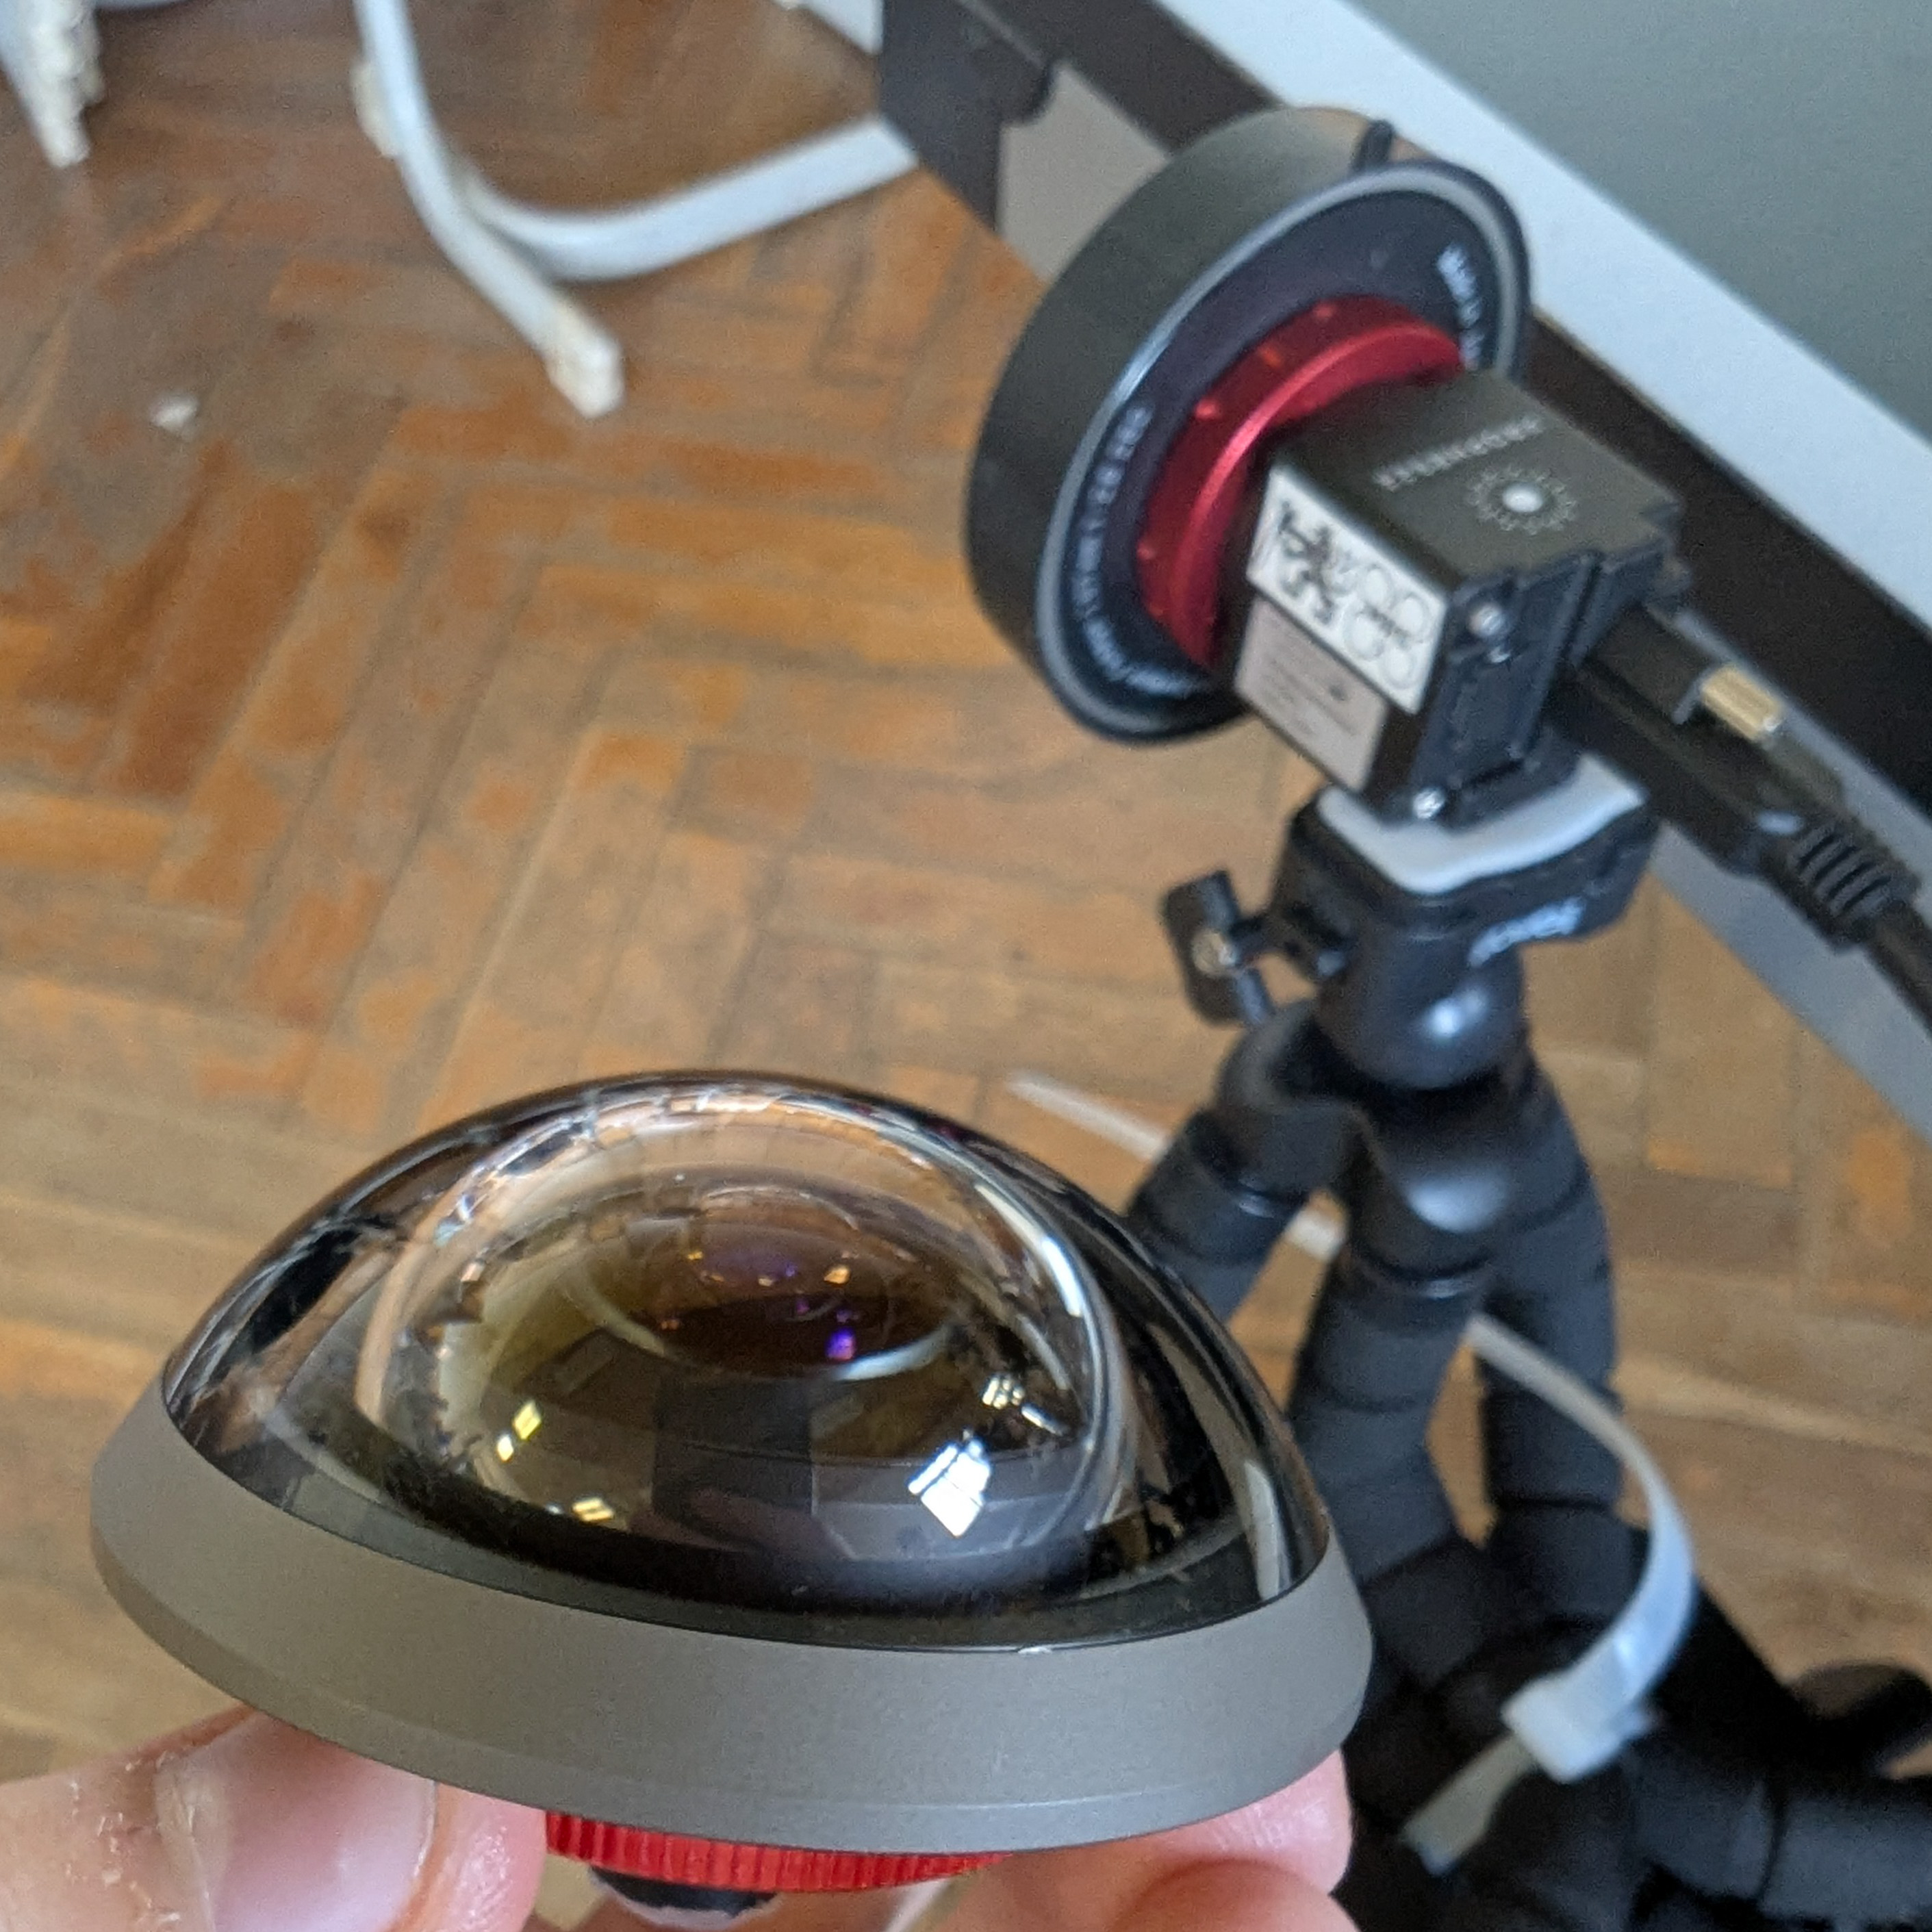
\includegraphics[width=0.4\textwidth]{./fig/photos/entaniya_280.jpg}
	  \label{fig:lens_2}
	}
	\caption{
		Lenses used during the calibration, a $187$ degree lens in \reffig{fig:lens_1} and Entaniya $280$ degree lens in \reffig{fig:lens_2}.
  }
	\label{fig:lenses}
\end{figure}

\section{Response data collection}

\subsection{Baseline}

The baseline experiment involved a static event-based camera mounted on a tripod, observing a stationary \ac{UAV} positioned at distances ranging from
$0.5$ m to $2.5$ m under controlled indoor lighting. The \ac{UAV}'s \ac{LED} markers were programmed to emit pulses of \ac{UV} light with modulation
frequencies ranging from $1$ Hz to $30$ kHz. No \ac{ROI} constraints were applied during these recordings.
This preliminary experiment revealed critical problems in the measuring technique:
\begin{itemize}
    \item Multiple visible \ac{LED}s: The camera captured the scene as a whole, with no isolation of individual light sources. This means that the results
    would not have a correct representation of a single light source, which would be influenced by other light sources from the remaining \ac{UAV}
    arms as well.
    \item Reflection artifacts: Reflections from walls and objects present in the scene acted as event-generating light sources, bouncing the light around,
    as seen on \reffig{fig:meas1}.
    This may confuse some blob detection algorithms for automatic \ac{LED} source location detection, which would be used in the analysis.
    \item Capturing of the whole scene: As the whole scene was captured, more post-processing would have been needed to analyze the recorded data and to investigate the relations of measured effects, for example a local \ac{ROI} filter could have been applied to \ac{LED} centers detected by a blob detection algorithm.
\end{itemize}

%This first experiment proved to be rather inefficient as the \ac{LED}s need to be isolated from each other's influence, which
%was not done properly at this time. This problem is partially solvable in the post-processing, by filtering out the events
%with \ac{ROI} filter usage (it is possible to filter the events by finding bounding boxes
%that encapsulate light sources, but on a more complex scene this approach becomes relatively hard).
%The other issue turned out to be the reflections of surrounding objects (as seen in \reffig{fig:meas1}), which caused
%another source of unwanted events in the recording, which may in turn confuse some blob detection methods.

\begin{figure}[H]
	\centering
	\subfloat[An event-camera view of the UAV with UV LEDs.] {
	  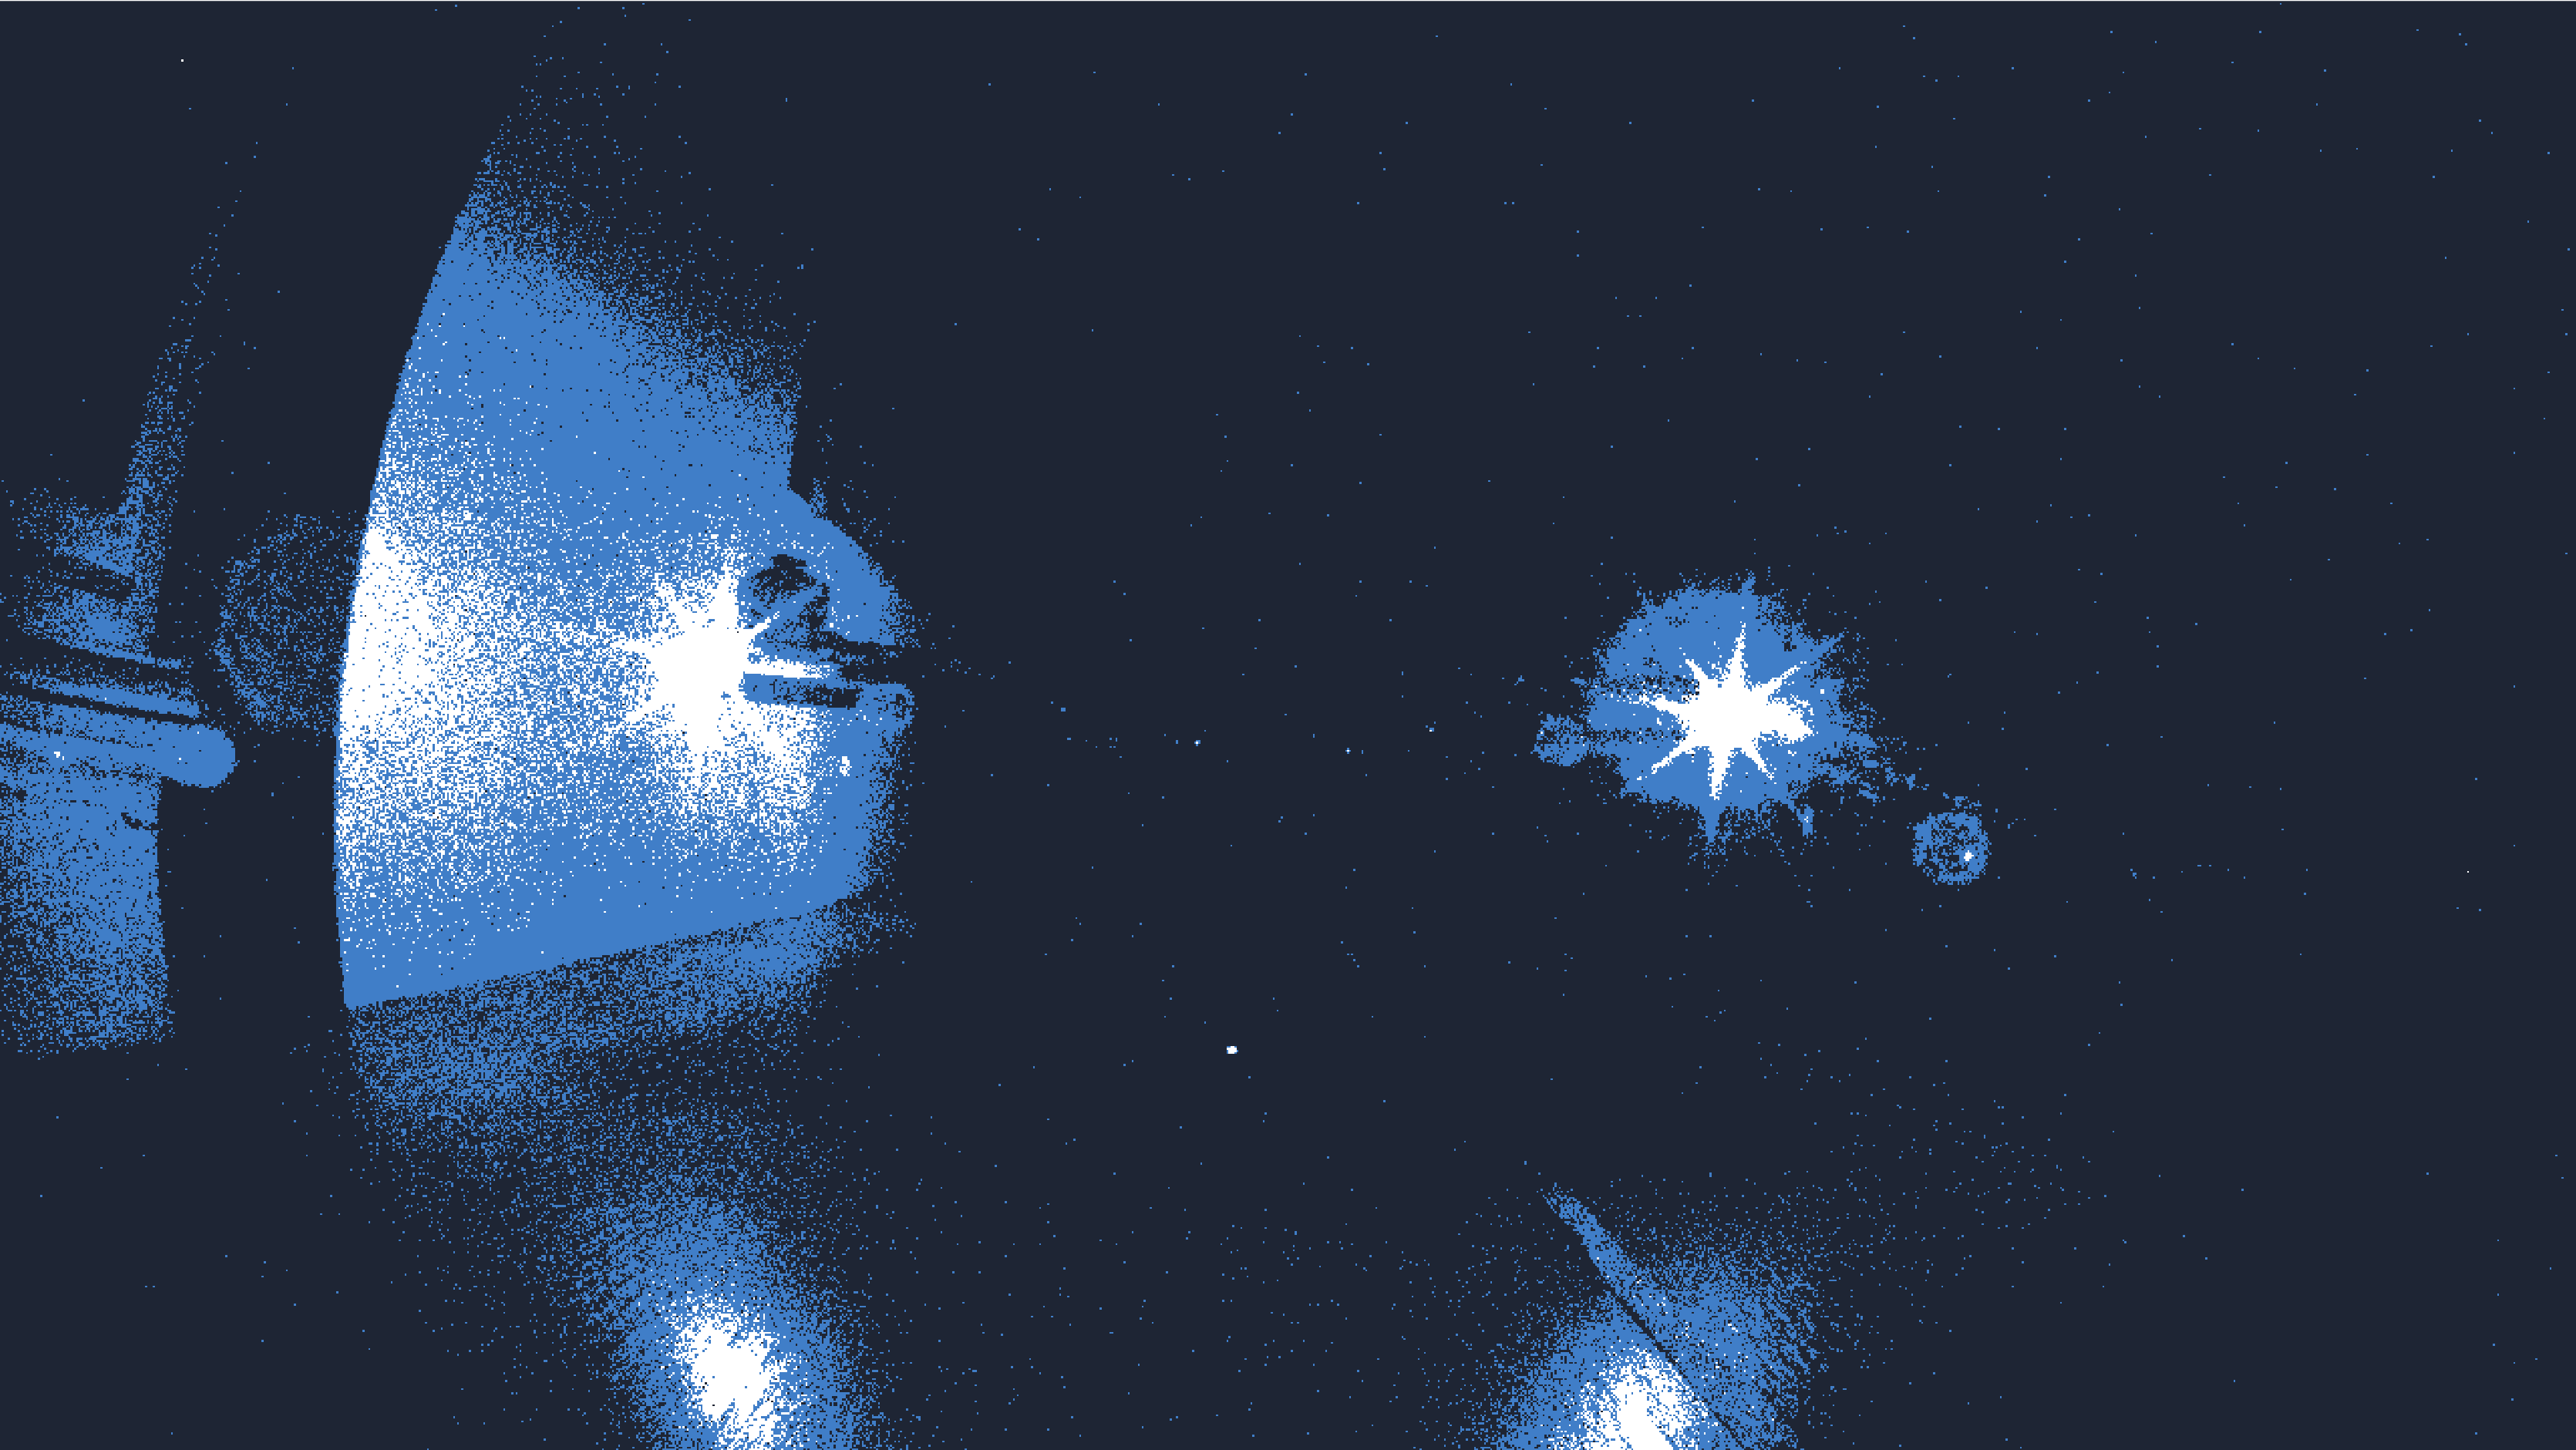
\includegraphics[width=0.5\textwidth]{./fig/photos/meas1.png}
	  \label{fig:meas1_e}
	}
	\subfloat[View of the experiment setup.] {
	  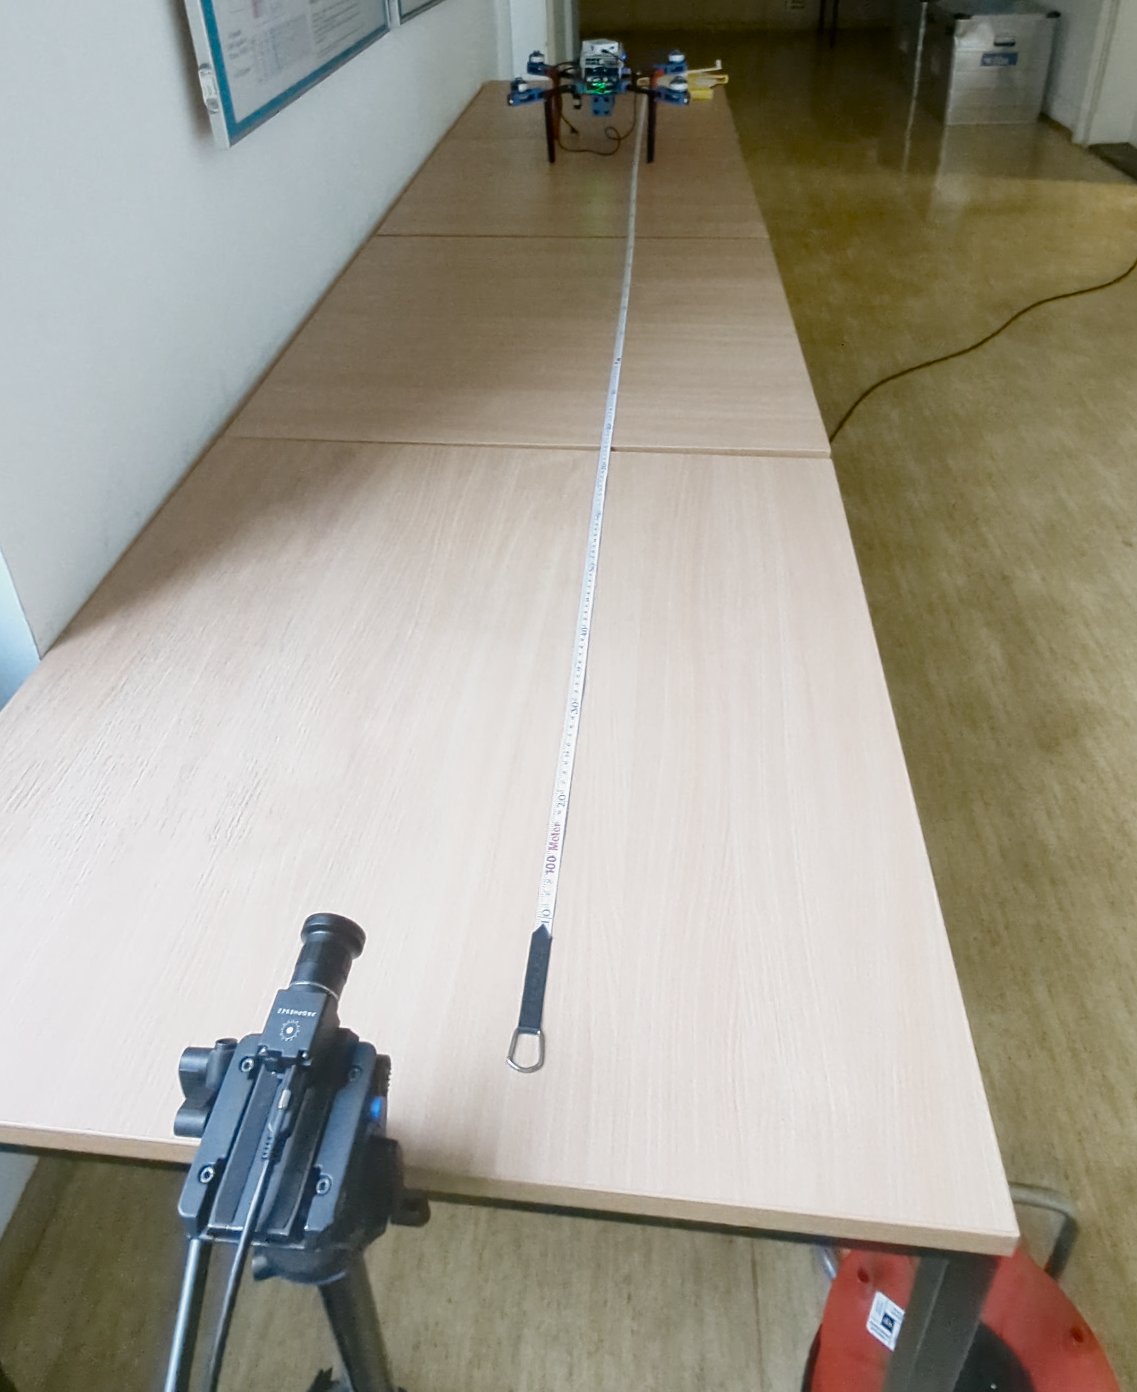
\includegraphics[width=0.3\textwidth]{./fig/photos/meas1_c.png}
	  \label{fig:meas1_c}
	}
	\caption{
  The setup for measuring the event-camera response with a EVK4 camera. Visible reflections from a wall can be seen on \reffig{fig:meas1}. The setup is shown on \reffig{fig:meas1_c}.
  }
	\label{fig:meas1}
\end{figure}


\subsection{Distance - frequency influence}

With the critical problems revealed in the previous experiment, only one light source consisting of 2 \ac{UV} \ac{LED}s at the end of the \ac{UAV} arm was turned on and
modulated at set frequencies.
Measurements were made in areas isolated by \ac{ROI} filter directly during recording on the hardware level, events were collected only in the
selected area around the and of the \ac{UAV} arm.
This time, the position of the \ac{UAV} was fixed relative to the camera on a blank background, with no wall reflections. The camera was placed on a tripod
and moved in increments of $0.2$ meters, starting from $1$ meter and ending at $3$ meters, with additional measurements made
at $4$ and $5$ meters.
The frequency range of the LED modulation was set in a range of $10$ Hz to $30$ kHz, with the blinking sequence set to $"0, 1"$.

\subsection{Rotation angle influence}

In addition to distance and frequency influence, the rotation angle influence was also explored to
verify the emitting characteristics of the light sources - if they can or cannot be considered Lambertian.
The \ac{UAV} was rotated at increments of $45$ degrees relative to the event-based camera, at distances of $0.5$, $1$ and $2$ meters,
with frequencies ranging from $10$ Hz to $10$ kHz and the blinking sequence was set to $"0, 1"$.

%\subsection{RSSR Data collection}

%TODO: Rewrite this section

%Another dataset was collected for the application of \ac{RSSR} \cite{sooyongrssr}, which we analyze more in \refchap{chap:rssr}.
%The data includes calibration data, which is necessary for the optical system parameter estimation. This calibration is done by
%recording a video using a calibration lattice of LEDs with known spacing, and observing the pattern distortion in the
%resulting video.
%The UAV was placed at increasing distances and various angles relative to the event-based camera, with the LEDs blinking at frequencies different from
%each other. 
%The blinking sequences were set to the following values:
%\begin{lstlisting}
%	led_1 = [0, 0, 0, 0, 0, 0, 0, 0, 1, 1, 1, 1, 1, 1, 1, 1]
%	led_2 = [0, 0, 0, 0, 1, 1, 1, 1, 0, 0, 0, 0, 1, 1, 1, 1]
%	led_3 = [0, 0, 1, 1, 0, 0, 1, 1, 0, 0, 1, 1, 0, 0, 1, 1]
%	led_4 = [0, 1, 0, 1, 0, 1, 0, 1, 0, 1, 0, 1, 0, 1, 0, 1]
%\end{lstlisting}
%with a common modulation frequency of $250$ Hz.
%This allows for the measurement of the ratio
%explain why to use the ratio, not the absolute value
%\footnote{Using the absolute value of the LED power is not suitable, as it also depends of the camera settings, surrounding
%environment and other factors. Finding such ratio (or property) that stays constant is crucial for correct distance estimation.}
%between the responses for each of the LEDs, which is necessary
%for the estimation of the UAV position using RSSR.


\section{Calibration data collection}

To facilitate calibration, a reference chessboard pattern with known square size is usually used, which offers high contrast between squares, making the square corners easily detectable.
Multiple images are usually taken, at various rotations and distances, to obtain good calibration results.
In our calibration procedure, we use a $5\times7$ lattice of UV LEDs, which are spaced 50 mm apart from each other. With this pattern, events are generated at the center of the
LEDs and can be detected by any kind of blob detector. The LED lattice is used, so the event-based camera can easily detect events from bright LEDs, as opposed to
the light being reflected from the chessboard pattern (which does not produce any light on its own).
The calibration lattice can be seen in \reffig{fig:lattice}.

\begin{figure}[H]
	\centering
	\subfloat[Calibration lattice] {
	  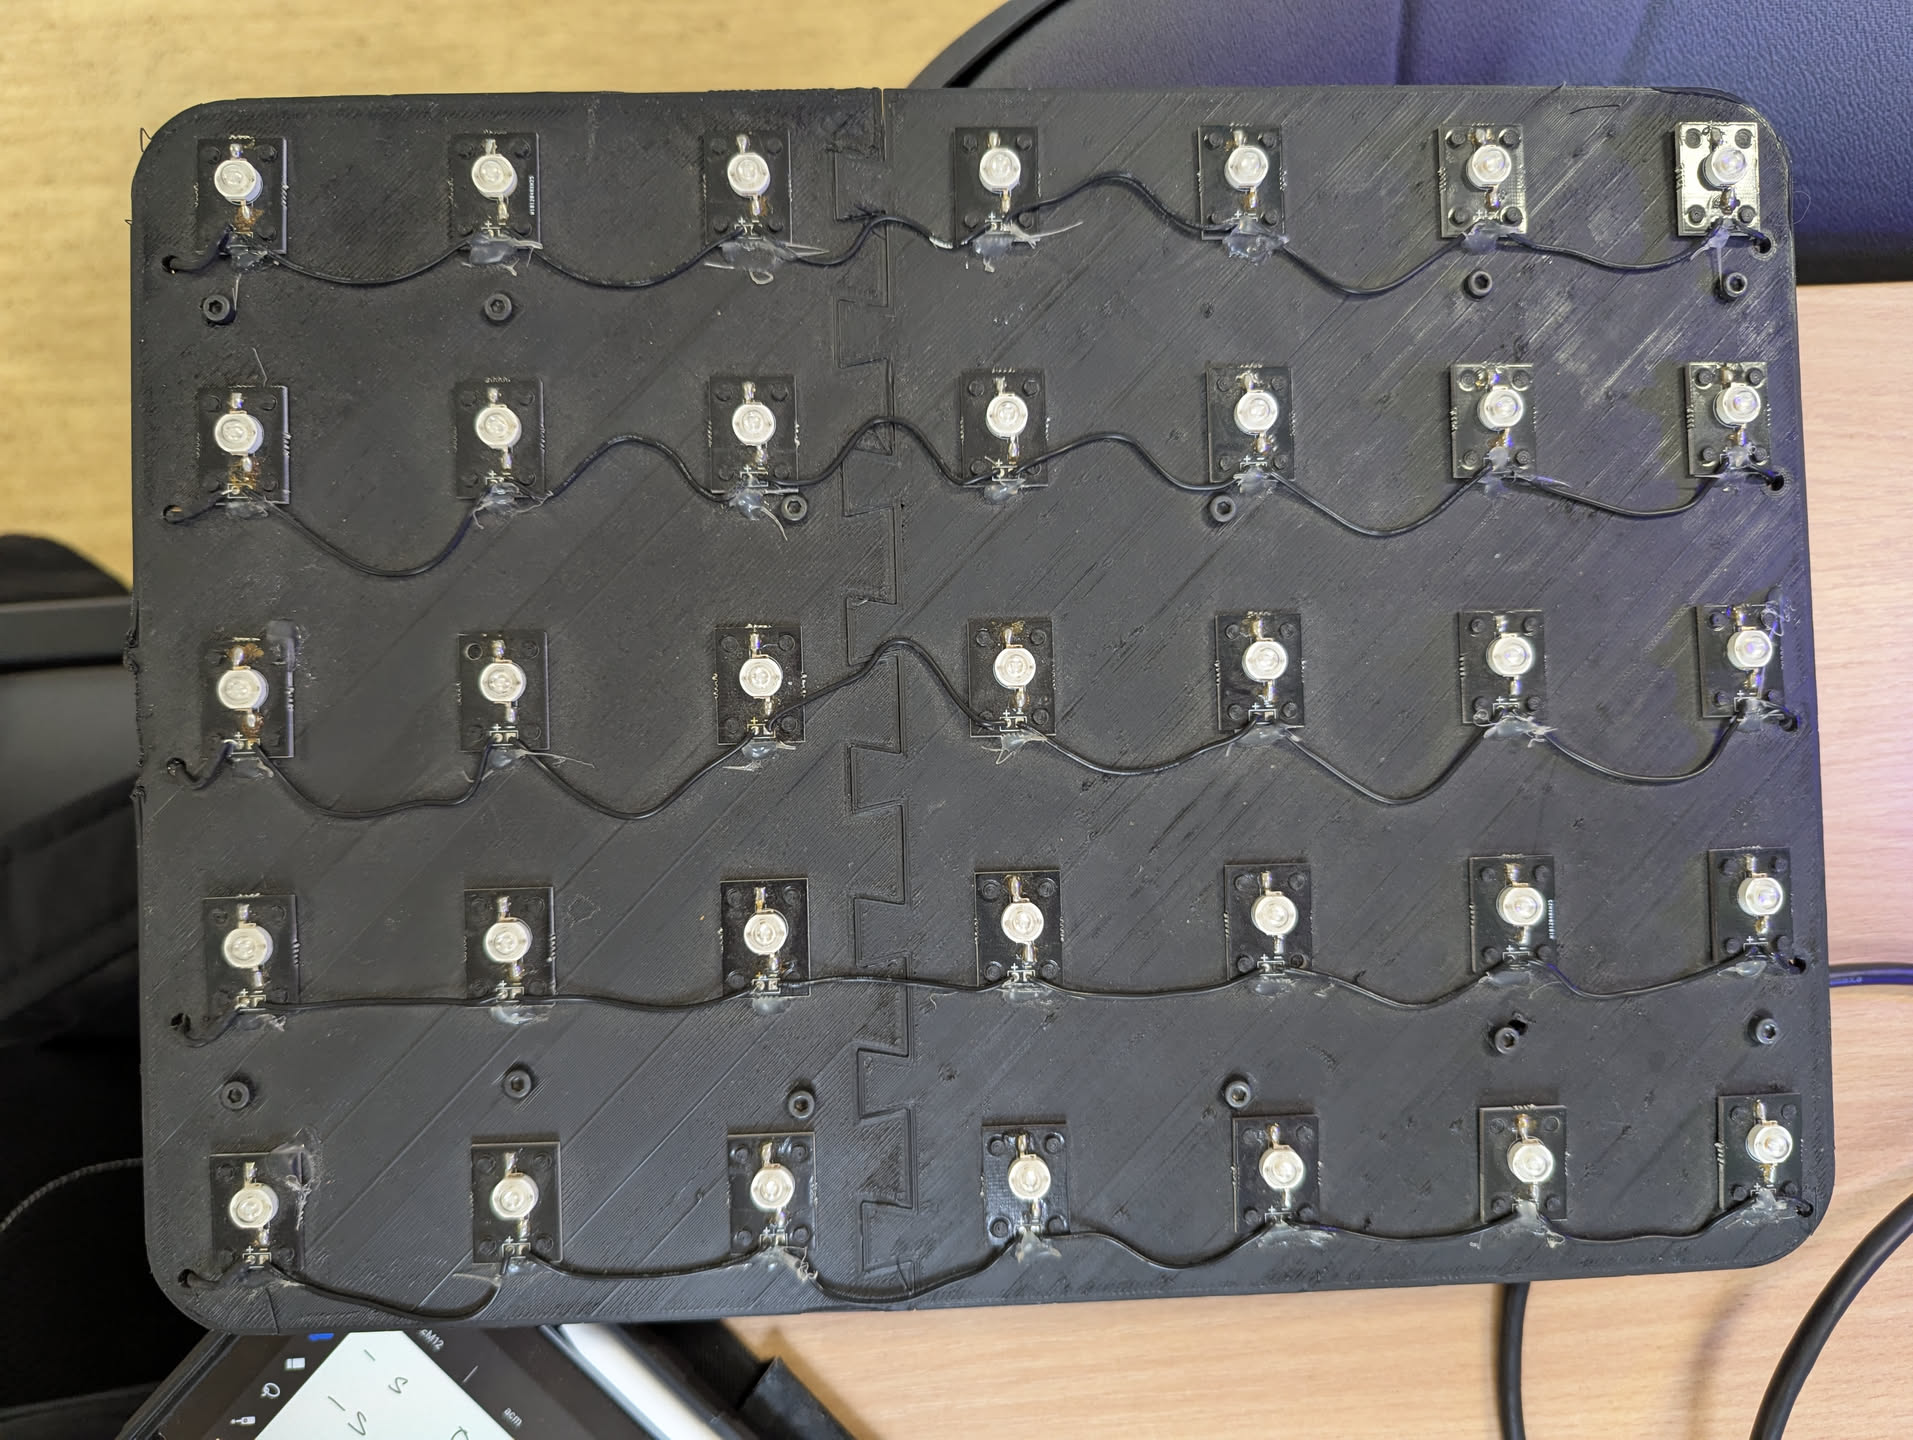
\includegraphics[width=0.4\textwidth]{./fig/photos/lattice.jpeg}
	  \label{fig:lattice_1}
	}
	\subfloat[Image from the event camera of the calibration lattice] {
	  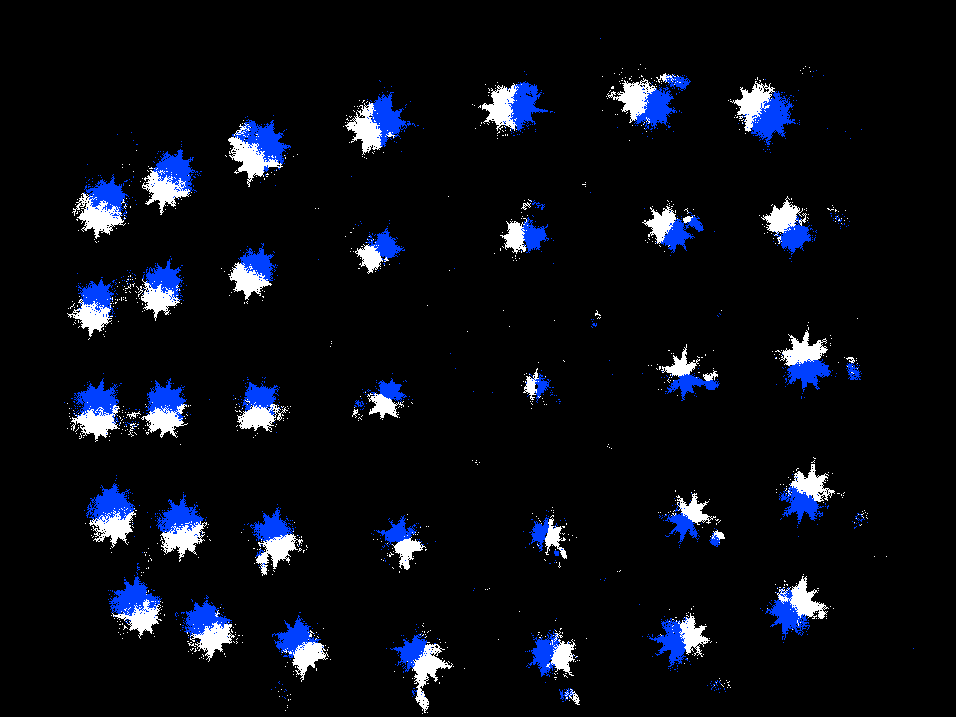
\includegraphics[width=0.4\textwidth]{./fig/photos/lattice_evs.png}
	  \label{fig:lattice_2}
	}
	\caption{
		Calibration lattice of $5\times7$ UV LEDs on \reffig{fig:lattice_1} and the events being produced when placed in front of the camera at \reffig{fig:lattice_2},
		with typical fish-eye lens distortion.
  }
	\label{fig:lattice}
\end{figure}
The downside of using an LED lattice instead of a chessboard pattern is that at a very high \ac{FOV}, the distortion of the fisheye lens sometimes does not allow
reliable detection of the exact center of the blobs (or which events correspond to which \ac{LED}), as can be seen at \reffig{fig:calibration_pattern_distorted}.
\begin{figure}[H]
  \centering
  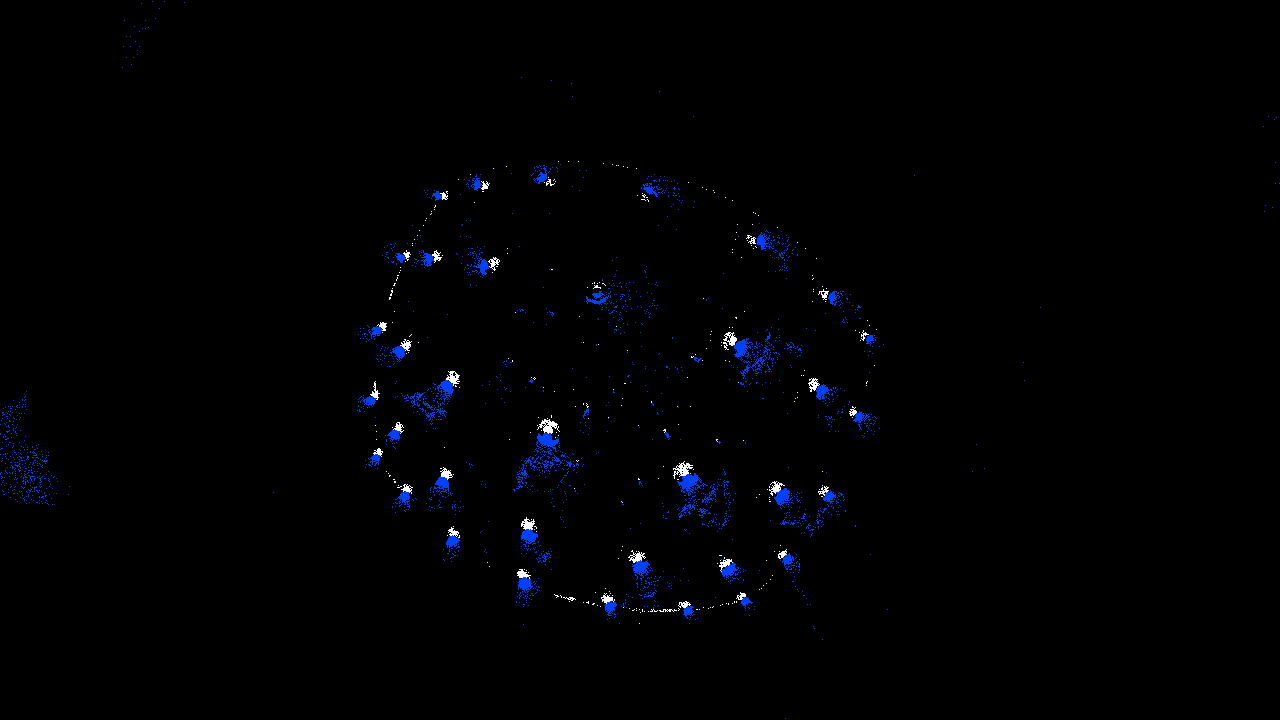
\includegraphics[width=0.6\textwidth]{./fig/photos/lattice_280.png}
  \caption{Calibration pattern with $5\times7$ lattice of UV LEDs, taken with a lens with Entaniya lens with \ac{FOV} of 280 degrees.}
  \label{fig:calibration_pattern_distorted}
\end{figure}

The implementation used for the calibration was a Python library \texttt{py-OCamCalib} \footnote{\texttt{py-OCamCalib} is available at \url{https://github.com/jakarto3d/py-OCamCalib}}.
As a regular image of a chessboard pattern was not used (required by the library), rather a recording of accumulated events on \ac{LED} grid, some data preprocessing had to be done beforehand.
For the purpose of this, a simple Python app had been written. An event raw recording was loaded, and events were accumulated over a select period of time.
The accumulated events were then saved to a grayscale image, where each pixel corresponded to the number of events that occurred in that
pixel (positive and negative) as in \ref{lst:accumulate}. The image was then normalized,
and the LED centers were detected using the \texttt{findContours} function of the OpenCV library, by finding the brightest points in the detected
contour area on the original grayscale image as shown in \ref{lst:blob_centers}.

\newpage
%\lstinputlisting[language=Python, caption={Accumulating events into a grayscale image}, label={lst:accumulate}]{./fig/code/accumulate.py}
\begin{algorithm}
\caption{Accumulating events into a grayscale image}
\label{alg:accumulate_events}
\begin{algorithmic}[1]
\Procedure{AccumulateEvents}{$raw\_file, start\_time\_us, acc\_time\_us, threshold$}
    \State $reader \gets \text{RawReader}(raw\_file)$
    \State $reader.\text{seek\_time}(start\_time\_us)$
    \State $height, width \gets reader.\text{get\_size}()$
    \State $pos\_accumulator \gets \text{zeros}((height, width), \text{dtype}=\text{uint16})$
    \State $neg\_accumulator \gets \text{zeros}((height, width), \text{dtype}=\text{uint16})$
    \State $end\_time\_us \gets start\_time\_us + acc\_time\_us$
    \While{$reader.\text{current\_time} < end\_time\_us$}
        \State $events \gets reader.\text{load\_delta\_t}(1000)$
        \If{$events$ is $\text{None}$}
            \State \textbf{break}
        \EndIf
        \For{each $event$ in $events$}
            \State $x, y, p, \_ \gets event$
            \If{$p > 0$}
                \State $pos\_accumulator[y, x] \gets pos\_accumulator[y, x] + 1$
            \Else
                \State $neg\_accumulator[y, x] \gets neg\_accumulator[y, x] + 1$
            \EndIf
        \EndFor
    \EndWhile
    \State $pos\_acc\_n \gets \text{normalize}(pos\_accumulator, \text{min}=0, \text{max}=255, \text{type}=\text{uint8})$
    \State $neg\_acc\_n \gets \text{normalize}(neg\_accumulator, \text{min}=0, \text{max}=255, \text{type}=\text{uint8})$
    \State $combined\_accumulator \gets \text{addWeighted}(pos\_acc\_n, 0.5, neg\_acc\_n, 0.5, 0)$
    \State \Return $combined\_accumulator$
\EndProcedure
\end{algorithmic}
\end{algorithm}

\lstinputlisting[language=Python, caption={Blob center detection in the grayscale image}, label={lst:blob_centers}]{./fig/code/blob_centers.py}
\newpage

The detected centers can then be manually labeled row-wise, in the same order in every image, so the calibration process can identify 
how the grid of points changes across the images, and thus calculate the lens distortion.
After this, the regular calibration script from \texttt{py-OCamCalib} can be used with the prelabeled grid points, the labeling of the LED centers can be seen in \reffig{fig:calibration_pattern_labeled}.

\begin{figure}[H]
  \centering
  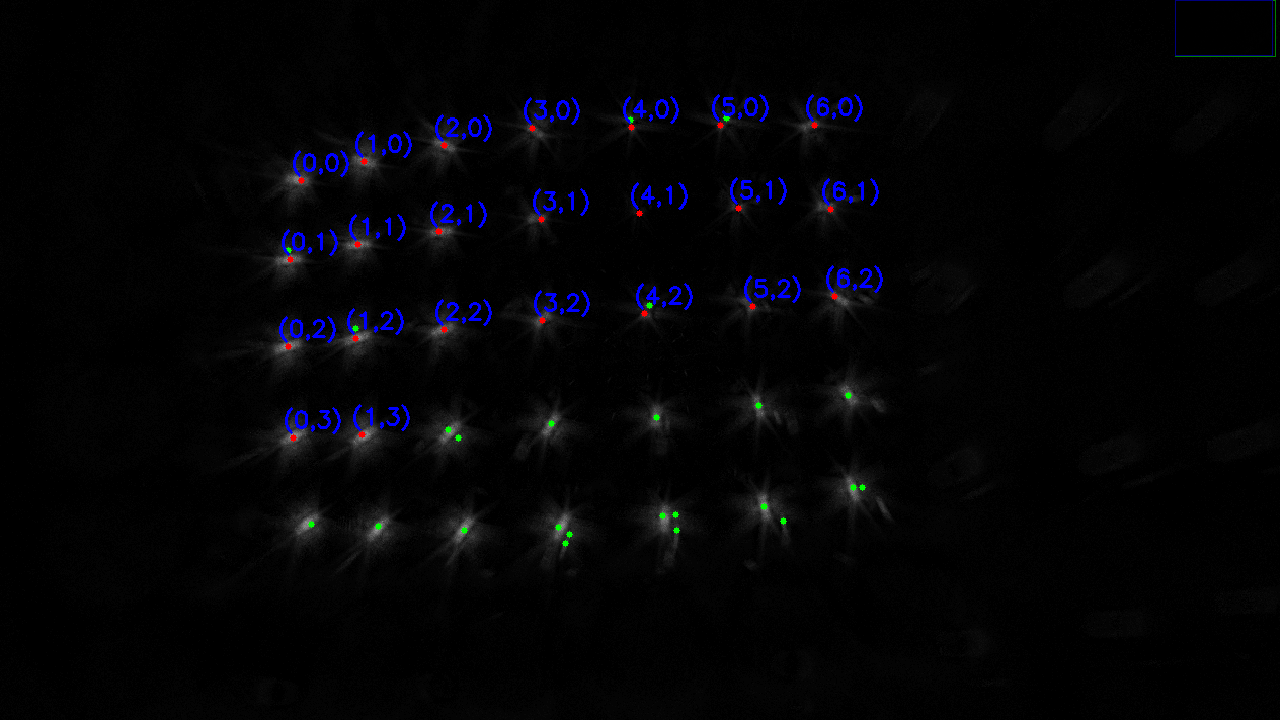
\includegraphics[width=0.7\textwidth]{./fig/photos/lattice_blobs.png}
  \caption{Calibration pattern with 5x7 lattice of UV LEDs, with the centers of the LEDs being labeled.}
  \label{fig:calibration_pattern_labeled}
\end{figure}

\section{ROS implementation}
To facilitate the deployment on real hardware, a \ac{ROS} \texttt{DistanceEstimator} node was implemented
\footnote{The source code of the distance estimator \ac{ROS} node is available at \url{https://github.com/kubakubakuba/ros-event-distance}}.
The functionality can be summarized with the flow chart
in
\reffig{fig:rosflow}.
\begin{figure}[H]
	\centering
	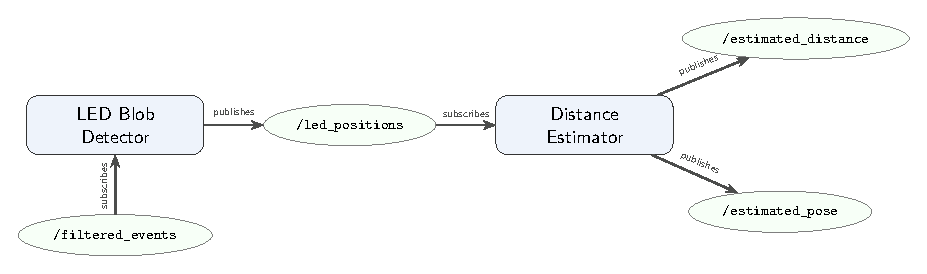
\includegraphics[width=1.0\textwidth]{./fig/tikz/rosflow.pdf}
	\caption{ROS distance estimation pipeline}
	\label{fig:rosflow}
\end{figure}
On the input, a filtered event stream is present, with filtering based on the known blinking frequencies of the \ac{LED} markers.
On these events, an image is integrated and a blob detection is run on top of it. The resulting blobs are marked as the \ac{LED} positions and passed 
on to the distance estimator, which uses a \ac{P3P} (or \ac{PnP} if all markers are visible) to estimate the pose of the \ac{UAV}. The distance estimator publishes the estimated pose as a quaternion, but also an estimated distance as a floating-point number.

\section{Stationary experiment\label{sec:stationary_experiment}}
An experiment with a stationary \ac{UAV} and event-based camera was conducted prior to the experiment with flying \ac{UAV}s to ensure functionality.
A \ac{UAV} was placed at the floor several meters from the camera and rotated around to obstruct one \ac{LED} in some measurements to test out \ac{P3P}. The \ac{LED} blinking frequencies were set to $\mathcal{F} = \{125, 250, 500, 1000\}$ Hz, and a blob detector was used to detect the centers of the visible blobs. The individual \ac{LED}s were identified by their visible
brightness differences (which were influenced by the event-based camera response to the blinking frequencies) and by the known physical structure of the \ac{UAV}. The view from the event-based camera can be seen on \reffig{fig:pnpuav}.
\begin{figure}[H]
	\centering
	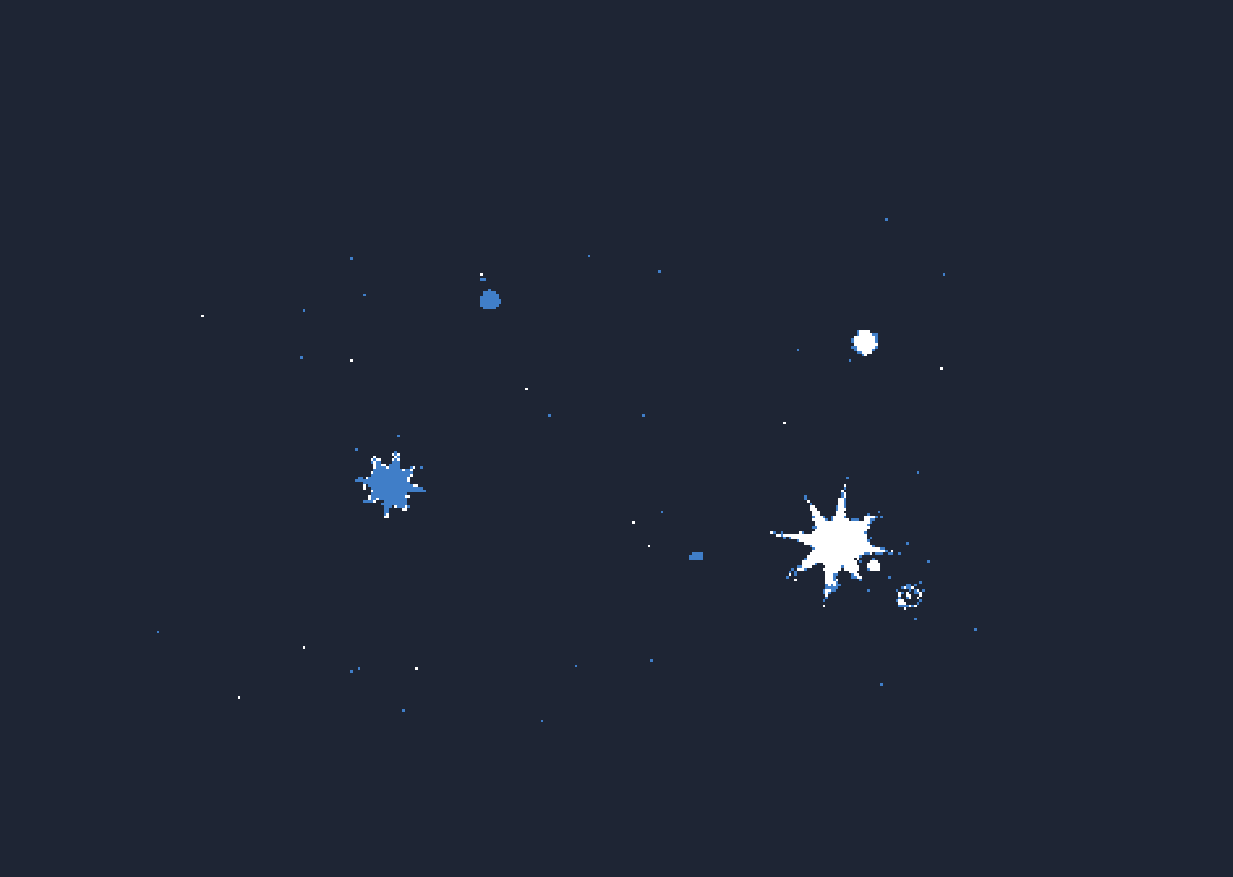
\includegraphics[width=0.65\textwidth]{./fig/photos/pnpmeas.png}
	\caption{Data from the stationary experiment}
	\label{fig:pnpuav}
\end{figure}

\section{Real-world experiment setup}

The real-world experiment was performed with two X500 \ac{UAV}s, each of them equipped with a Prophesee EVK4 event-based camera, one with a 2.5mm f/1.6
fisheye lens with an \ac{FOV} of roughly 187 degrees and the second one with Entaniya 1.07mm f/2.8 fisheye lens with an \ac{FOV} of 280 degrees.
Each UAV is also equipped with a Basler camera with a fisheye lens, to provide normal video signal that is recorded alongside the event stream
from the event-based camera.
Both cameras are connected to the onboard Intel NUC computer running the \ac{ROS} system, on which all the processing is done during the flight. Both 
\ac{UAV}s are also equipped with a \ac{RTK} module, which is used to localize the \ac{UAV}, and is used as ground truth data for the pose estimation.
The UVDAR blinking frequencies $\mathcal{F} = \{4.0, 2.0, 1.\overline{3}, 1.0\}$ (in kHz) were defined, where each of the arms were blinking at its assigned
frequency.
The measurements were collected during the \ac{MRS} Camp in Temešvár in August 2025, the \ac{UAV}s can be seen on \reffig{fig:uav33_37}.
\begin{figure}[H]
	\centering
	\subfloat[UAV33] {
	  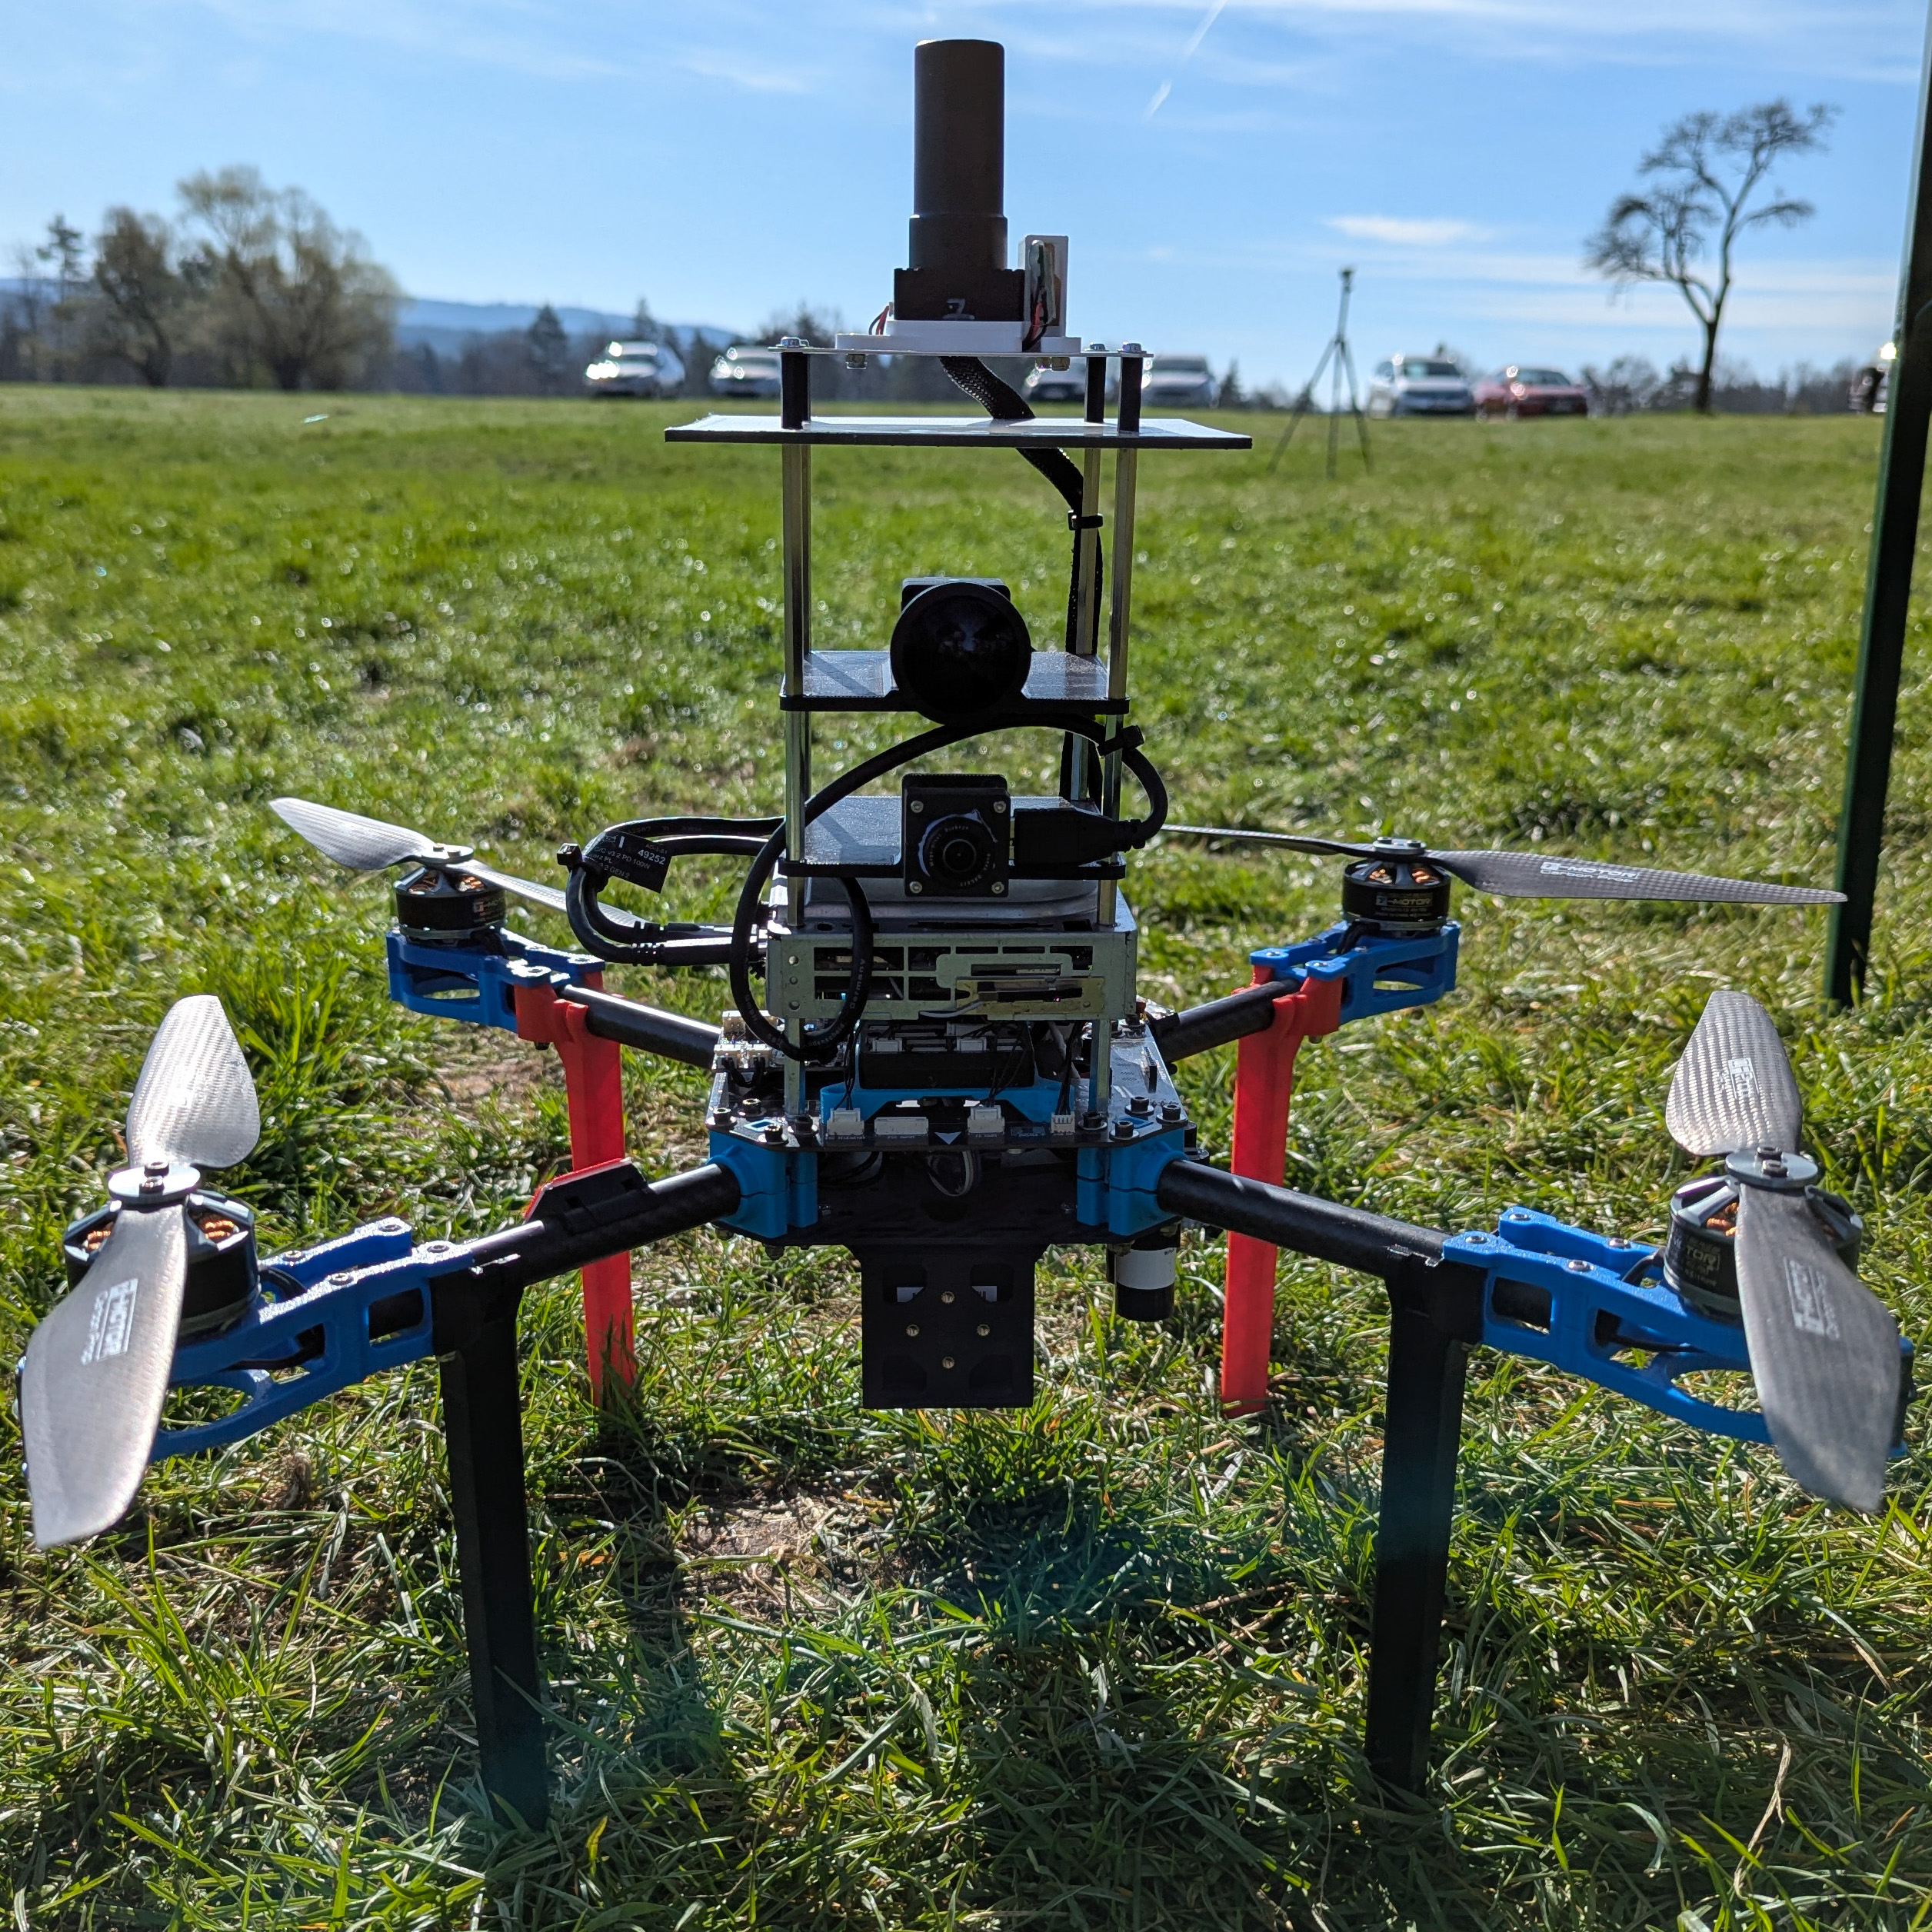
\includegraphics[width=0.4\textwidth]{./fig/photos/uav33.jpg}
	  \label{fig:uav33}
	}
	\subfloat[UAV37] {
	  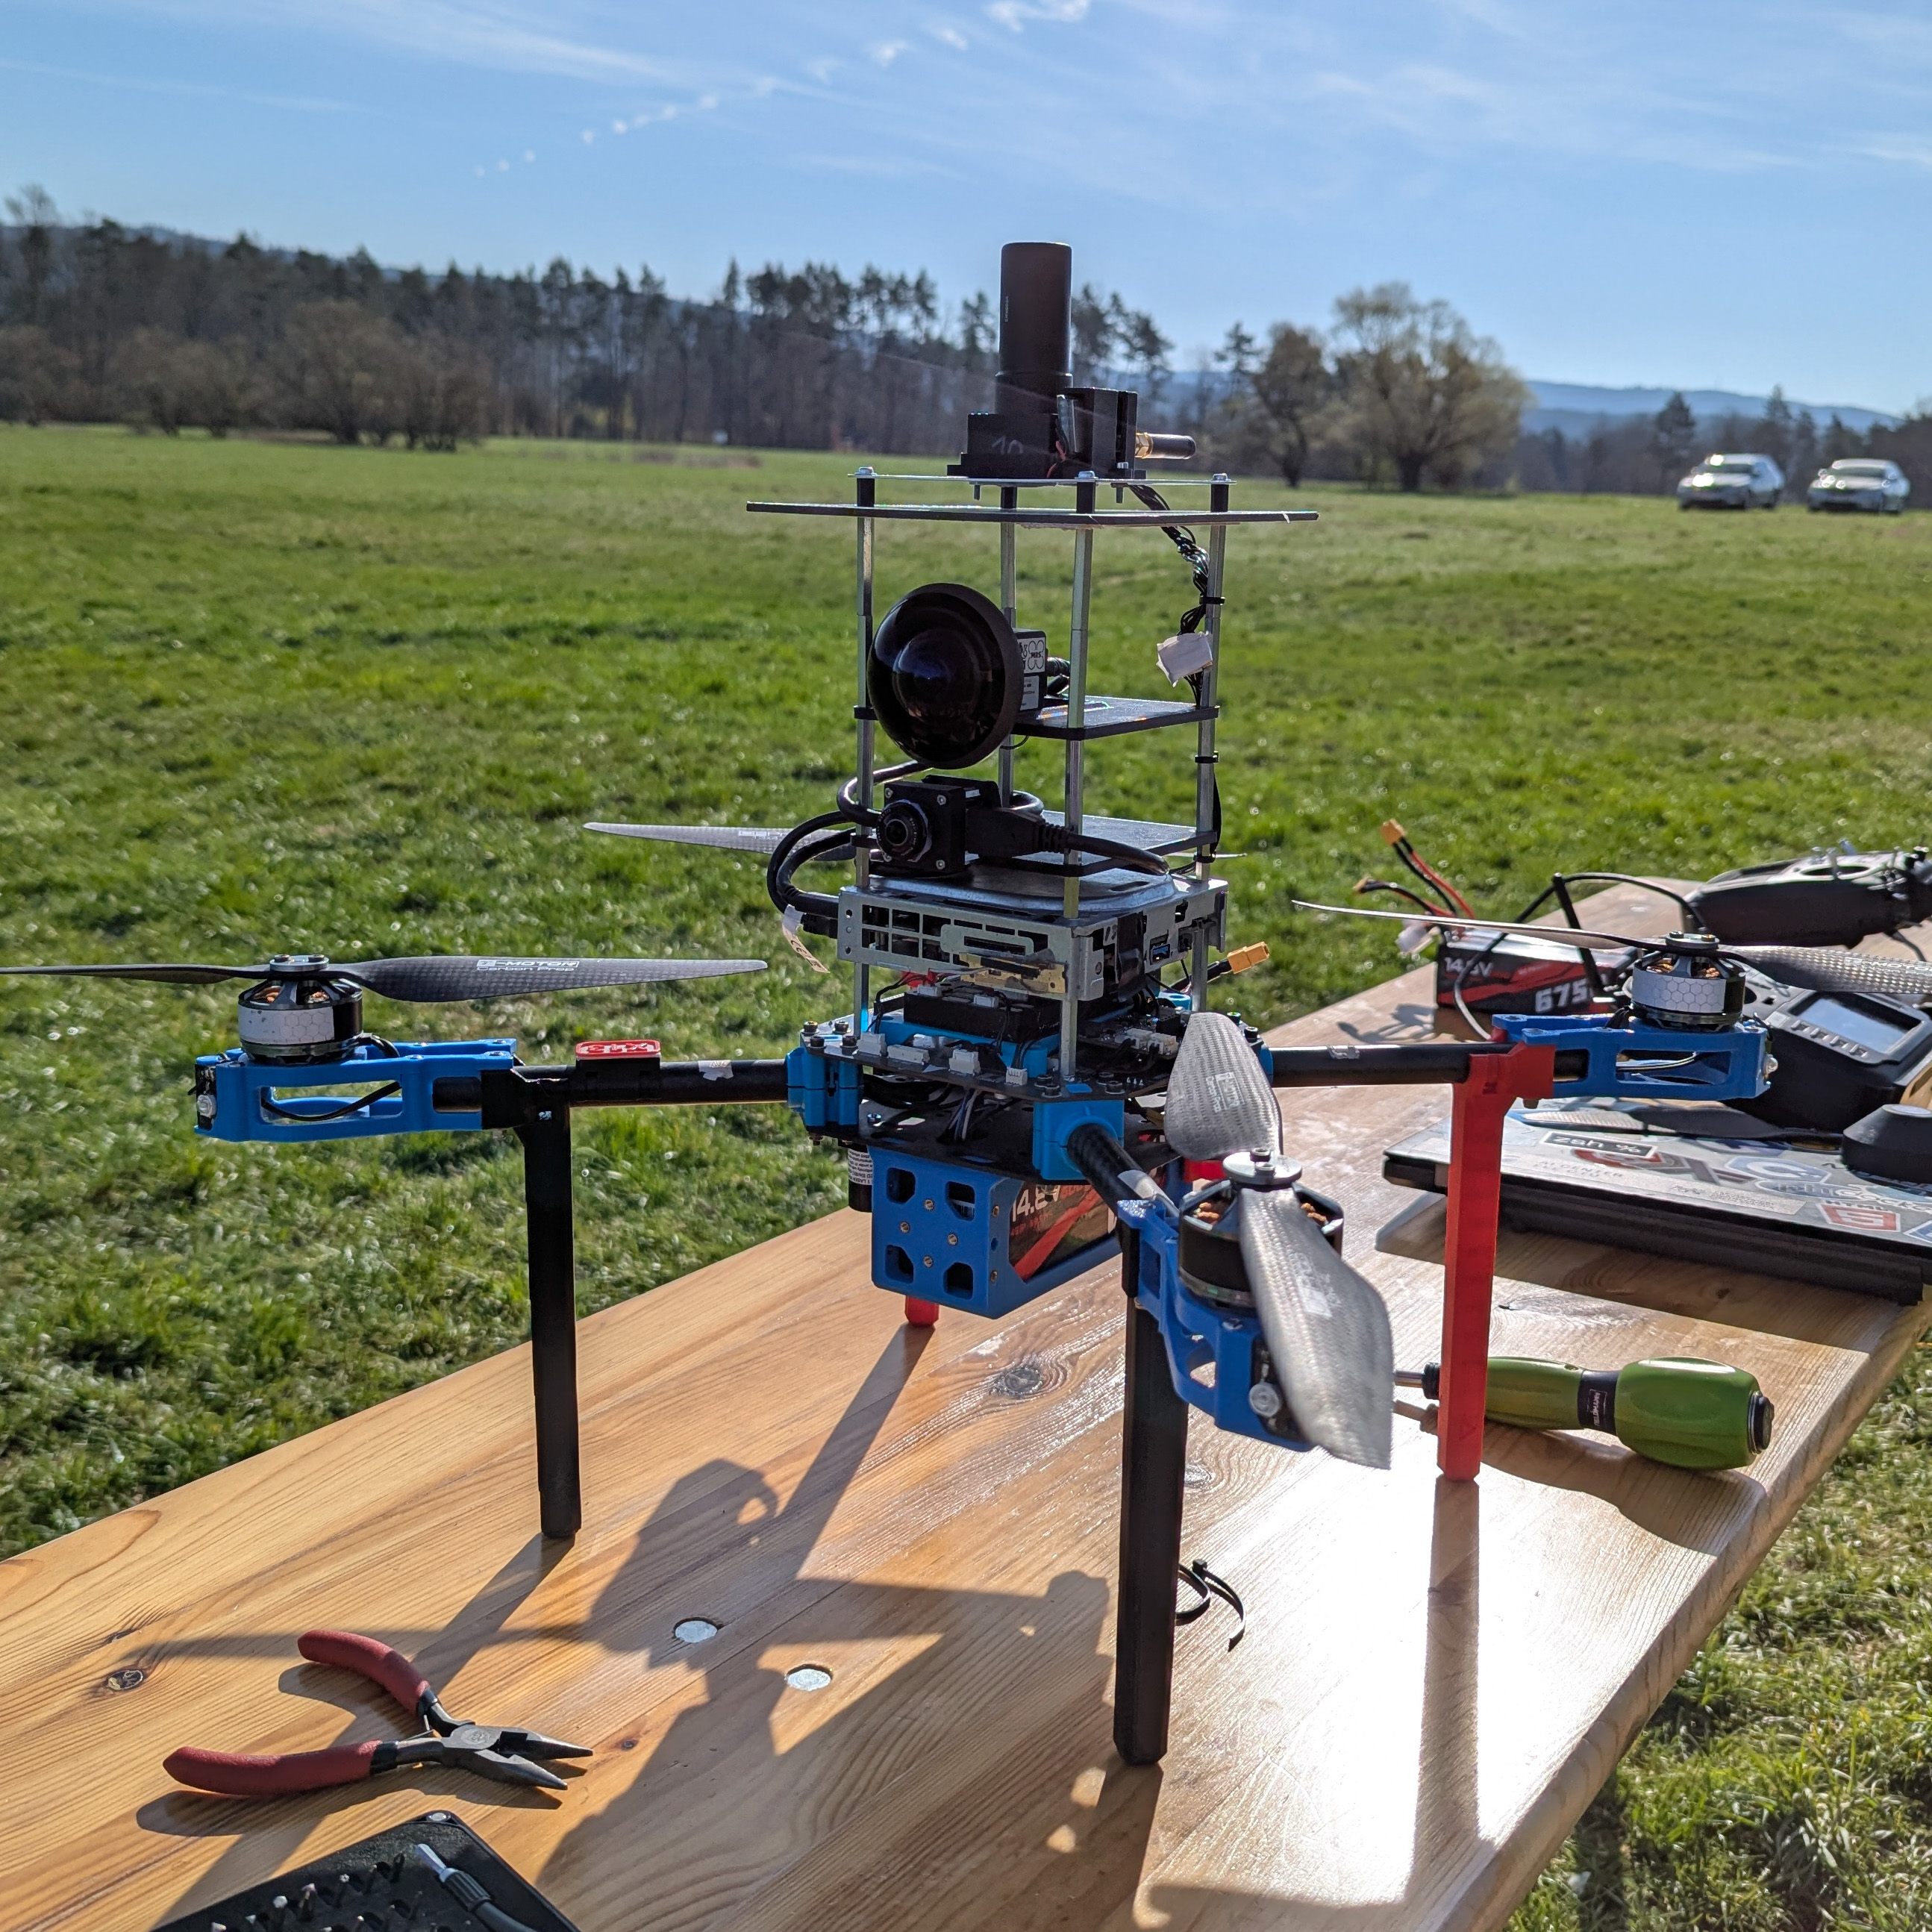
\includegraphics[width=0.4\textwidth]{./fig/photos/uav37.jpg}
	  \label{fig:uav37}
	}
	\caption{
		Two X500 UAVs, UAV33 on \reffig{fig:uav33} and UAV37 on \reffig{fig:uav37}.
  }
	\label{fig:uav33_37}
\end{figure}
Two pilots manually controlled the \ac{UAV}s, systematically varying the distance and angles between them to generate diverse measurement data during the experiment. All in-flight data, including sensor measurements and camera streams, were recorded in a \ac{ROS} bag file for subsequent analysis
in a simulated environment. In addition, raw event stream data from the event-based camera was also recorded and saved. The camera view from the UAV33
can be seen on \reffig{fig:exp1}. During the recording about $17$ million events were generated every second by each camera, which equates to a data
throughput of about $45$ MB per second per drone. Each raw recording is about $14$ gigabytes in size.

\begin{figure}[H]
	\centering
	\subfloat[Event-based camera output] {
	  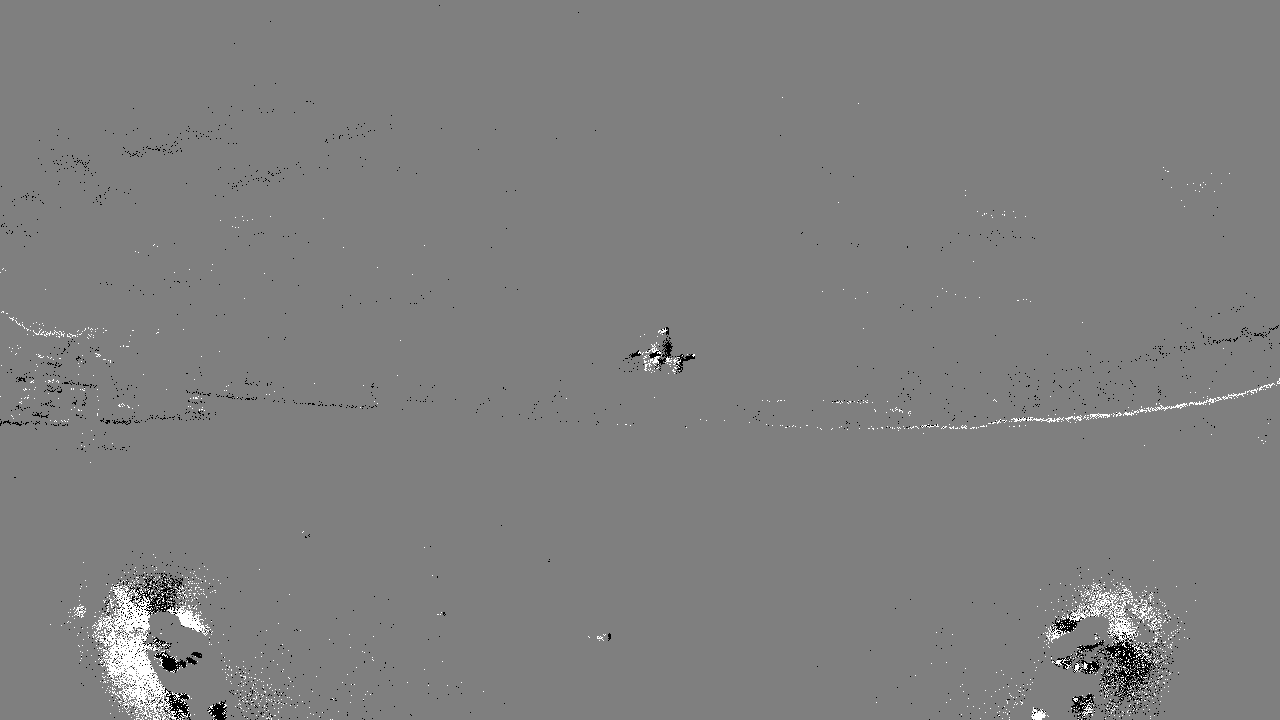
\includegraphics[width=0.50\textwidth]{./fig/photos/uav33_event.png}
	  \label{fig:exp1_event}
	}
	\subfloat[Basler camera output] {
	  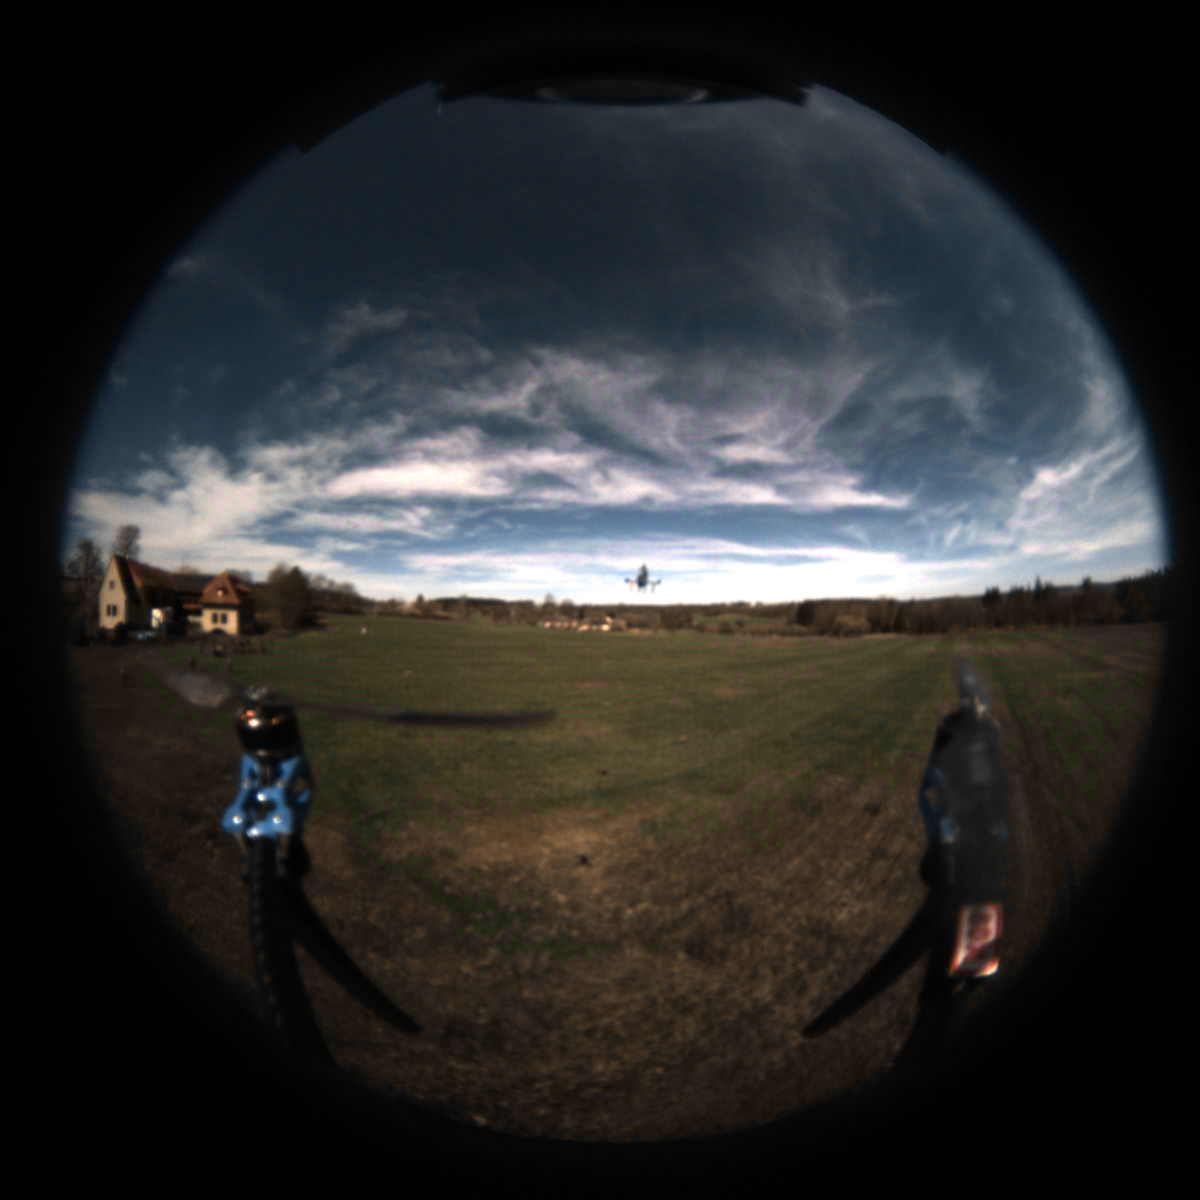
\includegraphics[width=0.282\textwidth]{./fig/photos/uav33_basler.png}
	  \label{fig:exp1_basler}
	}
	\caption{
		The view of the experiment from UAV33, with event data on \reffig{fig:exp1_event} and Basler camera view on \reffig{fig:exp1_basler}.
  }
	\label{fig:exp1}
\end{figure}

%\todo{SHOW MEASURED DATA FROM RQT}

%\todo{SHOW GNSS/ESTIMATION DIFFERENCES}

%\todo{SHOW THE RVIZ/RQTPLOT VISUALIZATION PIPELINE}